\documentclass[11pt]{article}
\usepackage[utf8]{inputenc}
\usepackage[T1]{fontenc}
\usepackage{lmodern}
\usepackage{amsmath,amssymb,amsthm}
\usepackage[margin=1.1in]{geometry}
\usepackage{hyperref}
\usepackage{booktabs}
\usepackage{pgfplots}
\pgfplotsset{compat=1.17}
\usepgfplotslibrary{fillbetween}
% Figures of the paper; data from fig/make_figdata.py. Colours: categorical slot 1 blue 2A78D6, slot 2 orange EB6834,
% slot 3 aqua 1BAF7A; text and axes in grey ink.
\definecolor{cblue}{HTML}{2A78D6}
\definecolor{corange}{HTML}{EB6834}
\definecolor{caqua}{HTML}{1BAF7A}
\definecolor{cink}{HTML}{52514E}
\definecolor{cgrid}{HTML}{D9D8D3}

% the tube: sections at t = 0.05, 0.25, 0.5, 0.75, 0.95 (fig/make_tube.py), light to dark in time
\definecolor{ct0}{HTML}{9EC5F4}
\definecolor{ct1}{HTML}{6DA7EC}
\definecolor{ct2}{HTML}{3987E5}
\definecolor{ct3}{HTML}{256ABF}
\definecolor{ct4}{HTML}{184F95}
\newcommand{\figtube}{%
\begin{tikzpicture}
\begin{axis}[width=0.8\textwidth, height=0.62\textwidth, xmin=-15, xmax=82, ymin=-12, ymax=78,
  xlabel={longitude (deg)}, ylabel={latitude (deg)}, axis line style={cink}, tick style={cink},
  label style={cink, font=\small}, tick label style={cink, font=\footnotesize}, grid=major,
  grid style={cgrid, very thin}, clip=true]
\addplot[ct0, line width=0.9pt] table {fig/fig_tube_t0.dat};
\addplot[ct1, line width=0.9pt] table {fig/fig_tube_t1.dat};
\addplot[ct2, line width=0.9pt] table {fig/fig_tube_t2.dat};
\addplot[ct3, line width=0.9pt] table {fig/fig_tube_t3.dat};
\addplot[ct4, line width=0.9pt] table {fig/fig_tube_t4.dat};
\addplot[corange, line width=1pt, dashed] coordinates {(60,-12) (60,78)};
\addplot[cink, line width=1.4pt] table {fig/fig_shape_twelfth.dat};
\addplot[only marks, mark=*, mark size=1.8pt, cink] table {fig/fig_tube_eight.dat};
\addplot[only marks, mark=x, mark size=3.5pt, line width=1pt, cink] coordinates {(60,0)};
\addplot[only marks, mark=*, mark size=2.2pt, caqua] coordinates {(0,0)};
\node[font=\footnotesize, caqua, anchor=north east] at (axis cs:-1,-1) {$E$};
\node[font=\footnotesize, corange, anchor=west] at (axis cs:61,72) {$I$};
\node[font=\footnotesize, cink, anchor=north west] at (axis cs:61,-1) {$C_{23}$};
\node[font=\footnotesize, ct0, anchor=west] at (axis cs:10.5,-6) {$t=0.05$};
\node[font=\footnotesize, ct4, anchor=west] at (axis cs:66,30) {$t=0.95$};
\end{axis}
\end{tikzpicture}}

\newcommand{\figshape}{%
\begin{tikzpicture}
\begin{axis}[width=0.95\textwidth, height=0.46\textwidth, xmin=-180, xmax=180, ymin=-90, ymax=90,
  xtick={-180,-120,-60,0,60,120,180}, ytick={-90,-45,0,45,90}, xlabel={longitude (deg)}, ylabel={latitude (deg)},
  axis line style={cink}, tick style={cink}, label style={cink, font=\small}, tick label style={cink, font=\footnotesize},
  grid=major, grid style={cgrid, very thin}, clip=true]
\foreach \i in {0,...,10} {\addplot[cink!45, line width=0.6pt] table {fig/fig_shape_copy\i.dat};}
\addplot[cblue, line width=1.6pt] table {fig/fig_shape_twelfth.dat};
% the plane I: meridians 60 and -120 deg
\addplot[corange, line width=1pt, dashed] coordinates {(60,-90) (60,90)};
\addplot[corange, line width=1pt, dashed] coordinates {(-120,-90) (-120,90)};
% collisions (equator at 180, 60, -60) and Euler points (0, 120, -120)
\addplot[only marks, mark=x, mark size=3.5pt, line width=1pt, cink] coordinates {(180,0) (-180,0) (60,0) (-60,0)};
\addplot[only marks, mark=*, mark size=2.2pt, caqua] coordinates {(0,0) (120,0) (-120,0)};
\node[font=\footnotesize, cblue, anchor=south east] at (axis cs:28,22) {$\gamma_8$};
\node[font=\footnotesize, caqua, anchor=north] at (axis cs:0,-5) {$E$};
\node[font=\footnotesize, corange, anchor=west] at (axis cs:62,70) {$I$};
\node[font=\footnotesize, cink, anchor=north] at (axis cs:60,-5) {$C_{23}$};
\end{axis}
\end{tikzpicture}}

\newcommand{\figlogic}{%
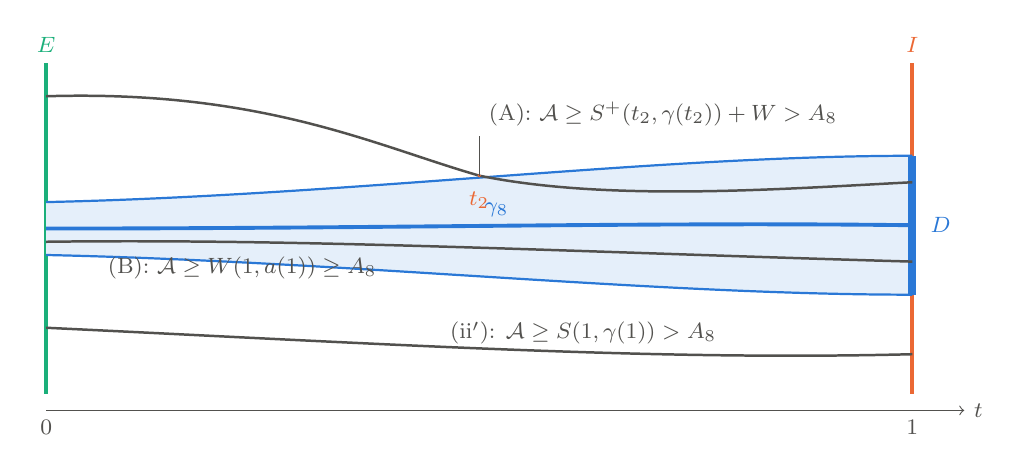
\begin{tikzpicture}[x=11cm, y=4.2cm, font=\footnotesize]
% axes: time 0 (E) to 1 (I)
\draw[cink, ->] (0,-0.05) -- (1.06,-0.05) node[right] {$t$};
\node[cink, below] at (0,-0.05) {$0$}; \node[cink, below] at (1,-0.05) {$1$};
\draw[caqua, line width=1.4pt] (0,0) -- (0,1) node[above] {$E$};
\draw[corange, line width=1.4pt] (1,0) -- (1,1) node[above] {$I$};
% the tube (closed label sets mapped forward), its end disc D on I
\fill[cblue!12] (0,0.42) .. controls (0.35,0.40) and (0.7,0.30) .. (1,0.30) -- (1,0.72)
  .. controls (0.7,0.72) and (0.35,0.60) .. (0,0.58) -- cycle;
\draw[cblue, line width=0.8pt] (0,0.42) .. controls (0.35,0.40) and (0.7,0.30) .. (1,0.30);
\draw[cblue, line width=0.8pt] (0,0.58) .. controls (0.35,0.60) and (0.7,0.72) .. (1,0.72);
\draw[cblue, line width=3pt] (1,0.30) -- (1,0.72);
\node[cblue, right] at (1.01,0.51) {$D$};
% the eight
\draw[cblue, line width=1.4pt] (0,0.5) .. controls (0.4,0.5) and (0.7,0.52) .. (1,0.51);
\node[cblue, above] at (0.52,0.505) {$\gamma_8$};
% (B): stays in the tube, starts on E
\draw[cink, line width=0.9pt] (0,0.46) .. controls (0.3,0.47) and (0.6,0.43) .. (1,0.40);
\node[cink, anchor=west] at (0.06,0.38) {(B): $\mathcal A\ge W(1,a(1))\ge A_8$};
% (A): leaves the tube; last exit t_2
\draw[cink, line width=0.9pt] (0,0.9) .. controls (0.25,0.92) and (0.38,0.75) .. (0.5,0.66)
  .. controls (0.65,0.58) and (0.85,0.62) .. (1,0.64);
\fill[corange] (0.5,0.66) circle (0.6pt);
\node[cink, anchor=south west] at (0.5,0.78) {(A): $\mathcal A\ge S^+(t_2,\gamma(t_2))+W>A_8$};
\draw[cink, very thin] (0.5,0.66) -- (0.5,0.78);
\node[corange, anchor=north] at (0.5,0.64) {$t_2$};
% (ii'): ends on I outside D
\draw[cink, line width=0.9pt] (0,0.2) .. controls (0.4,0.15) and (0.7,0.1) .. (1,0.12);
\node[cink, anchor=south] at (0.62,0.12) {(ii$'$): $\mathcal A\ge S(1,\gamma(1))>A_8$};
\end{tikzpicture}}

\newcommand{\figcover}{%
\begin{tikzpicture}
\begin{axis}[width=0.9\textwidth, height=0.5\textwidth, xmin=0.37, xmax=1.32, ymin=-3.3, ymax=1.55,
  xlabel={$\theta$}, ylabel={$\kappa=M/\sqrt{\varepsilon}$}, axis line style={cink}, tick style={cink},
  label style={cink, font=\small}, tick label style={cink, font=\footnotesize},
  colormap={eps}{HTML(0cm)=(CDE2FB); HTML(1cm)=(9EC5F4); HTML(2cm)=(6DA7EC); HTML(3cm)=(3987E5);
    HTML(4cm)=(256ABF); HTML(5cm)=(184F95); HTML(6cm)=(0D366B)},
  point meta min=-3, point meta max=-0.699, colorbar, colorbar style={ylabel={$\log_{10}\varepsilon_{\rm top}$},
  ylabel style={cink, font=\footnotesize}, tick label style={cink, font=\footnotesize}, width=0.25cm}]
\addplot graphics[xmin=0.37, xmax=1.32, ymin=-3.3, ymax=1.55] {fig/fig_cover.png};
\end{axis}
\end{tikzpicture}}

\newcommand{\figcellmin}{%
\begin{tikzpicture}
\begin{semilogyaxis}[width=0.9\textwidth, height=0.42\textwidth, xmin=-3.2, xmax=11.2,
  xlabel={$\sigma$ (cell layer)}, ylabel={$\min F$ per cell},
  axis line style={cink}, tick style={cink}, label style={cink, font=\small},
  tick label style={cink, font=\footnotesize}]
\addplot[name path=hi, draw=none, forget plot] table[x=sigma, y=fmax] {fig/fig_cellmin_layers.dat};
\addplot[name path=lo, draw=none, forget plot] table[x=sigma, y=fmin] {fig/fig_cellmin_layers.dat};
\addplot[cblue!15, forget plot] fill between[of=hi and lo];
\addplot[cblue, line width=1.2pt] table[x=sigma, y=fmin] {fig/fig_cellmin_layers.dat};
\addplot[cink, line width=0.8pt, dashed] table[x=sigma, y=fmed] {fig/fig_cellmin_layers.dat};
\end{semilogyaxis}
\end{tikzpicture}}


\newtheorem{theorem}{Theorem}
\newtheorem{proposition}[theorem]{Proposition}
\newtheorem{lemma}[theorem]{Lemma}
\newtheorem{corollary}[theorem]{Corollary}
\theoremstyle{definition}
\newtheorem{definition}[theorem]{Definition}
\newtheorem{remark}[theorem]{Remark}
\newcommand{\TODO}[1]{\textbf{[TODO: #1]}}

\title{The figure eight is the unique action minimiser\\ in its symmetry class}
\author{Oleksii Stavriianov\thanks{Independent researcher. ORCID \href{https://orcid.org/0009-0002-8504-3626}{0009-0002-8504-3626}, \texttt{oleksii.stavriianov@gmail.com}}}
\date{Version 1.3, November 2026}

\begin{document}
\maketitle

\begin{abstract}
In the planar three-body problem with equal masses and Newtonian attraction, Chenciner and Montgomery proved in 2000
that the action has a collision-free minimiser among loops with the symmetry group $D_6$ of the figure eight. Whether
this minimiser is unique has been open since; in 2002 Chenciner listed it among the global questions that ``seem to be
out of reach at the moment''. We prove that it is unique: the minimisers are exactly the figure eight and its images
under the isometries of the plane that preserve the symmetry class. Equivalently, the twelfth of the eight joining an
Euler configuration to an isosceles one is the unique minimiser, up to the mirror, of the action among paths between
these two sets of configurations, and it is nondegenerate. The proof is a calibration argument in the shape space: a piecewise polynomial
subsolution of the Hamilton-Jacobi equation bounds the action of paths that leave a tube around the eight, and a field
of extremals with no focal points calibrates the paths that stay in it. The finitely many inequalities this requires
are verified in interval arithmetic. The verification is packaged as a certificate, read as untrusted data by a
separate checker that recomputes every inequality and builds the covering itself; a mutated certificate is rejected.
The subsolution has $13\,248$ cells ($1.3\cdot10^9$ interval sub-boxes); the certificate has $11\,556$ leaves for the
field, $2\,190$ further leaves for the boundary records and $230$ boxes near the end, and the checker runs in about
13 hours on a laptop.
\end{abstract}

\section{Introduction}

\paragraph{The question.} Chenciner and Montgomery \cite{CM} found the figure-eight solution of the equal-mass planar
three-body problem, seen numerically by Moore \cite{Moore}, as a minimiser of the action
$\mathcal A=\int (K+U)\,dt$ over loops with a symmetry group isomorphic to $D_6$; they showed that a minimiser has no
collision and lies on an eight-shaped curve. Much is known about the numerically found orbit: existence, local uniqueness among
solutions and convexity of the lobes by a computer-assisted proof \cite{KZ}; convexity analytically \cite{FM}; KAM
stability by computer-assisted proofs \cite{KS,KS17}; its dynamical properties numerically \cite{Simo}; numerically,
its Morse indices and strict local minimality in its symmetry class \cite{HuSun,FFO18,Fenucci}; the families of
rotating eights that bifurcate from it \cite{CFM}; and it is the end of the continuation from the Lagrange triangle
in Marchal's conjecture \cite{CGHLM}. Whether the minimiser is unique has been asked since \cite{CM}. It is Question 1 of \cite{ChTaiyuan}:
``but is it unique ? Numerical evidence by Carles Sim\'o in [S1] suggests unicity of the minimizer'' ([S1] is \cite{Simo}); in Chenciner's
ICM address \cite[p.~291]{ChICM}: ``Two global questions seem to be out of reach at the moment: unicity and possible
extra symmetries of minimizers''; and \cite[\S6]{FM}: ``Showing the unicity of the Newtonian eight remains an open
problem''. Kapela and Zgliczy\'nski \cite[\S8]{KZ} list it among the open questions and propose to build ``rigorous
numerics for variational methods''; it is stated as open in \cite[Remark~4.16]{BFT} and \cite{CGHLM} as well. For the strong
force $1/r^2$, uniqueness was proved by Montgomery \cite{Mpants}. This paper answers the question for the Newtonian
eight in its symmetry class.

\paragraph{Main result.}
\begin{theorem}\label{thm:main}
In the planar three-body problem with masses $1,1,1$ and potential $U=\sum_{i<j}1/r_{ij}$, let $\mathcal H$ be the space
of $H^1$ loops of period $T$ with the symmetry group of \cite{CM} (collisions allowed; the group of order $12$ generated
by the two symmetries $\mathfrak s$ and $\mathfrak r$ of Section~\ref{sec:setting}, called $D_6$ in \cite{CM} and
$D_{12}$ in \cite{BFT}). The action on $\mathcal H$ attains its minimum exactly at four loops: the figure eight $x_8$,
its rotation by $\pi$, and the mirror images of these two (the images of $x_8$ under the isometries of the plane that
preserve $\mathcal H$).
\end{theorem}
Here $x_8$ is the orbit enclosed by the interval Newton (Krawczyk) computation of Section~\ref{sec:eight}; that it
coincides with the Chenciner-Montgomery minimiser is a consequence of the theorem, not an assumption.
As in \cite{CM} (see also \cite{FM}), minimality in $\mathcal H$ is equivalent to minimality of the twelfth of the loop
between an Euler (collinear, one body at the midpoint) configuration and an isosceles one (Figure~\ref{fig:shape}); we
prove Theorem~\ref{thm:main} in this form (Theorem~\ref{thm:twelfth}). The proof also gives the value of the minimum,
a gap for the competitors that leave a tube around the eight, in the sense of a lift to the field (Corollary~\ref{cor:gap}), and the nondegeneracy of
the minimiser: Morse index and nullity $0$ in $\mathcal H$ (Corollary~\ref{cor:nondeg}).

\begin{figure}[t]\centering
\figshape
\caption{The figure eight on the shape sphere (longitude and latitude of $x/|x|$, Section~\ref{sec:setting}). Bold: the
twelfth $\gamma_8$ from the Euler point $E$ (dots: the three Euler configurations) to the plane $I$ of isosceles
shapes (dashed: its two meridians); thin: its eleven images under the symmetry group, which close up into the loop.
Crosses: binary collisions; $C_{23}$ lies in $I$.}\label{fig:shape}
\end{figure}

\paragraph{Method and plan.} The proof is a calibration (field of extremals) argument in the reduced shape space, in
the spirit of the Weierstrass sufficiency theory, made global by an exit-time argument. Section~\ref{sec:setting}
reduces Theorem~\ref{thm:main} to paths $\gamma$ in $\mathbb R^3$ from a ray $E$ to a plane $I$. Section~\ref{sec:proof}
proves the reduced theorem by a sufficient criterion (Theorem~\ref{thm:criterion}) with three ingredients and a short
list of computer-verified statements (Table~\ref{tab:obligations}):
\begin{itemize}
\item a piecewise polynomial subsolution $S$ of the Hamilton-Jacobi equation, built from $E$, bounds from below the
action of any path up to any time (Section~\ref{sec:subsolution});
\item a family of extremals issuing from $I$ (the \emph{I-field}) covers a tube around the eight's twelfth with no
focal points; its value $W$ calibrates every path as long as it stays in the tube (Section~\ref{sec:field});
\item a path that leaves the tube pays at least $S+W$ at its last exit, and this exceeds the action $A_8$ of the eight
(Section~\ref{sec:eight}) on the whole tube boundary; paths ending outside the tube, and the start on $E$, are handled
by inequalities on $I$ and on $E$ (Section~\ref{sec:boundary}).
\end{itemize}
Each verified statement is a finite list of strict inequalities on boxes, checked in outward-rounded interval
arithmetic; Section~\ref{sec:cons} draws the consequences, Section~\ref{sec:checker} describes how the statements are
checked, and Section~\ref{sec:scope} states the scope and compares with other approaches.

\paragraph{Computation and its checking.} The search that produced the boxes is not part of the proof. Its output is a
\emph{certificate}: a list of boxes and the hashes of the input files. A separate checker reads the certificate as
untrusted data, recomputes every inequality, and builds the covering of the parameter domain itself, so that the
correctness of the proof rests on the checker and not on the search. The checker shares with the search the interval
arithmetic, the Taylor integrator and the evaluators, but not the bookkeeping (which boxes, which cover, which records),
where the errors of a search typically live (Section~\ref{sec:checker}). It rejects every
mutated certificate we tried (a removed box, a lowered bound, an oversized box, a wrong hash, a removed slab box, a
falsified record). The subsolution inequality, which carries the smallest margins, was also re-checked with an
independent implementation in Arb ball arithmetic. The code and the certificate are available at
\href{https://doi.org/10.5281/zenodo.24248043}{doi:10.5281/zenodo.24248043}.

\paragraph{Related work.} Variational existence proofs in the $n$-body problem show that minimisers under symmetry
constraints are free of collisions, in general by Marchal's averaging argument \cite{Marchal,FT}, or by comparing a
lower bound for the action of colliding paths with the action of a test path, analytically in
\cite{Chen08,Shibayama14}; a computer-assisted variational existence proof for choreographies is \cite{ABT}. These
results give existence, not uniqueness. Hamilton-Jacobi and weak KAM methods have been used analytically in the
$n$-body problem \cite{MV20}. Polynomial subsolutions of a Hamilton-Jacobi-Bellman equation as certified lower bounds
of a value function are used in optimal control \cite{LHPT}; this is the closest methodological relative of the
subsolution used here, which is piecewise polynomial and verified in interval arithmetic. For some symmetry classes the minimisers are known to be homographic (Lagrange) solutions
\cite{BFT}. To our knowledge, the present result is the first uniqueness theorem for a non-homographic action
minimiser of the Newtonian three-body problem in a symmetry class, and the proof the first computer-assisted
calibration argument for a periodic orbit of the $n$-body problem. For the larger loop space used by Liang, Xia and
Zhou \cite{LXZ}, our result covers only the $D_6$-equivariant sector of their hypothesis (Section~\ref{sec:cons}).

\section{Setting}\label{sec:setting}
This section turns Theorem~\ref{thm:main} into a statement about paths in $\mathbb R^3$ (Theorem~\ref{thm:twelfth}) and
records the one inequality on which every calibration below rests.

\subsection{Shape space}
We use the reduced shape space of the equal-mass planar problem in Hopf coordinates $x\in\mathbb R^3$ (zero angular
momentum, centre of mass at the origin), with
\[
  L(x,v)=\frac{|v|^2}{8|x|}+U(x),\qquad H(x,p)=2|x|\,|p|^2-U(x),\qquad
  U(x)=\sum_{k=1}^{3}\bigl(|x|-u_k\cdot x\bigr)^{-1/2},
\]
and the collision directions $u_3=(-1,0,0)$, $u_{1,2}=(\tfrac12,\pm\tfrac{\sqrt3}2,0)$. The metric
$g=|dx|^2/(4|x|)$ is the cone metric over the round sphere of radius $\tfrac12$ (the shape sphere); it is not flat.
$U$ is homogeneous of degree $-\tfrac12$ and is $+\infty$ on the three collision rays $\{x=|x|u_k\}$ and at the total
collision $x=0$. Explicitly, for positions $q_1,q_2,q_3\in\mathbb C$ with centre of mass $0$, let
$z_1=\tfrac1{\sqrt2}(q_2-q_1)$, $z_2=\sqrt{\tfrac23}\,(q_3-\tfrac{q_1+q_2}2)$, so that $K=\tfrac12(|\dot z_1|^2+|\dot z_2|^2)$,
and $x=(|z_1|^2-|z_2|^2,\ 2\operatorname{Re}z_1\bar z_2,\ 2\operatorname{Im}z_1\bar z_2)$. Then $|x|=|z_1|^2+|z_2|^2$ is the
moment of inertia, $r_{ij}^2=|x|-u_k\cdot x$ ($\{i,j,k\}=\{1,2,3\}$), so $U=\sum_{i<j}1/r_{ij}$, and for zero angular
momentum $K=|\dot x|^2/(8|x|)$: the shape action is the physical action, with no constant.

The Euler configurations with body $3$ at the midpoint form the ray $E=\{\rho e_1:\rho\ge0\}$; the isosceles
configurations with apex body $1$ ($r_{12}=r_{13}$) form the plane $I=\operatorname{span}(e_I,e_Z)$,
$e_I=(\tfrac12,\tfrac{\sqrt3}2,0)$, $e_Z=(0,0,1)$, with unit normal $n_I=(\tfrac{\sqrt3}2,-\tfrac12,0)$. The mirror
$x_3\mapsto-x_3$ preserves $U$, $E$ and $I$.

\subsection{Reduction to the twelfth}
The symmetry group of \cite{CM} is generated by
\[
(\mathfrak s\cdot x)(t)=(\Sigma q_3,\Sigma q_1,\Sigma q_2)(t-T/6),\qquad (\mathfrak r\cdot x)(t)=(-q_1,-q_3,-q_2)(-t),
\]
with $\Sigma$ the reflection in the vertical axis; it has order $12$ and acts on $\mathbb R/T\mathbb Z$ as a dihedral
group. The reductions below are standard.
\begin{enumerate}
\item \emph{Centre of mass.} For equal masses $K(q)=K(q-c)+\tfrac32|\dot c|^2$ with $c$ the centre of mass, the
potential is translation invariant, and $q-c$ lies in $\mathcal H$ again (the generators act linearly on positions and
commute with removing the common translation). So the action of $q-c$ is at most that of $q$, with equality iff
$\dot c=0$; the symmetry $\mathfrak r$ forces $c(t)=-c(-t)$, so a constant $c$ is $0$.
\item \emph{Fundamental domain.} The time-reversing elements $\mathfrak r$ and $\mathfrak r\mathfrak s$ fix $t=0$ and
$t=-T/12$. The configurations fixed by $\mathfrak r$ are the Euler configurations with one body at the midpoint (any
orientation), those fixed by $\mathfrak r\mathfrak s$ the isosceles ones with their axis on the horizontal axis (both
orientations, collinear ones included). In shape space, after relabelling, these sets are the ray $E$ and the whole
plane $I$. The interval $[-T/12,0]$ is a fundamental domain; every $H^1$ path from the isosceles set to the Euler set
extends to a loop in $\mathcal H$ by $x(g\cdot t)=g\cdot x(t)$ for the twelve elements $g$ of the group acting on
$\mathbb R/T\mathbb Z$ (the images of $[-T/12,0]$ tile the circle, and the definitions agree at the common end points
because the end configurations are fixed by $\mathfrak r$ and $\mathfrak r\mathfrak s$); the loop is $H^1$ and
$\mathcal A(x)=12\,\mathcal A_{1/12}(x|_{[-T/12,0]})$ \cite{CM,FM}. Reversing time, the twelfth becomes a path from the Euler set to the isosceles set, the orientation used
below.
\item \emph{Angular momentum.} For an $H^1$ path of centred configurations, $K=K_{\rm shape}+L^2/(2|x|)$ a.e.\ on
$\{x\neq0\}$, and a path that sits at total collision on a set of positive measure has infinite action, so
$\{t:x(t)=0\}$ is a null set and integrating the identity over $\{x\ne0\}$ loses nothing. The two fixed
subspaces project onto $E$ and onto the whole of $I$. Hence the action of any competitor is at least the action of its
shape projection, a path from $E$ to $I$, with equality iff the angular momentum vanishes a.e.; in the equality case
the configuration path is the horizontal lift of its shape path, determined up to the rotation by $\pi$ by the end
condition.
\item \emph{Time.} The Newtonian scaling $t\mapsto\lambda t$, $x\mapsto\lambda^{4/3}x$ (shape coordinates are quadratic
in the positions) multiplies the action by $\lambda^{1/3}$; we fix the duration of the twelfth to $1$.
\item \emph{Regularity.} A finite-action shape path is absolutely continuous, also through $x=0$
($|\dot x|=2\sqrt{|x|}$ times the cone speed), and spends a null set of times on the collision rays.
\end{enumerate}
The images of a minimiser under the rotation by $\pi$ and under the reflections of the plane in the two axes are again
minimisers; a general rotation does not preserve $\mathcal H$. The four loops of Theorem~\ref{thm:main} are the two
horizontal lifts, which differ by the rotation by $\pi$, of each of the two shape minimisers below. So
Theorem~\ref{thm:main} follows from:

\begin{theorem}\label{thm:twelfth}
Among finite-action paths $\gamma:[0,1]\to\mathbb R^3$ with $\gamma(0)\in E$ and $\gamma(1)\in I$, the action
$\mathcal A(\gamma)=\int_0^1L(\gamma,\dot\gamma)\,dt$ has exactly two minimisers: the eight's twelfth $\gamma_8$ and
its mirror image.
\end{theorem}

\subsection{Calibration along a path}
For $q,v\in\mathbb R^3$, Young's inequality gives
\begin{equation}\label{eq:young}
q\cdot v\le 2|x|\,|q|^2+\frac{|v|^2}{8|x|},\qquad\text{with equality iff } v=4|x|\,q .
\end{equation}
Hence, if $W$ is a $C^1$ solution of the backward Hamilton-Jacobi equation $W_t=2|x||\nabla W|^2-U$, then
$-\frac{d}{dt}W(t,\gamma(t))\le L(\gamma,\dot\gamma)$ a.e.\ along every absolutely continuous path, with equality
iff $\dot\gamma=-4|\gamma|\nabla W$. Likewise, if $S$ is a $C^1$ \emph{subsolution} of the forward equation,
$S_t+2|x||\nabla S|^2\le U$, then $\frac{d}{dt}S(t,\gamma(t))\le L$ a.e. The rest of the paper constructs such an $S$
(only Lipschitz) from $E$ and such a $W$ from $I$, and proves Theorem~\ref{thm:twelfth} from them.

\section{The proof modulo the computer-verified statements}\label{sec:proof}
This section proves Theorem~\ref{thm:twelfth} from the statements of Table~\ref{tab:obligations}, each introduced where
it is used; Sections~\ref{sec:eight} to~\ref{sec:boundary} then say how each statement is verified, and
Proposition~\ref{prop:checker} that the checker verifies all of them.

\begin{table}[h]\centering\footnotesize
\renewcommand{\arraystretch}{1.15}
\begin{tabular}{@{}p{1.7cm}p{5.6cm}p{3.0cm}p{3.6cm}@{}}\toprule
& statement & checked by & smallest margin \\ \midrule
\multicolumn{4}{@{}l}{\emph{the eight and the tube}}\\
(K), (K1) & the eight's label: unique zero of the shooting map in a box; $A_8\in[A_8]$ & Krawczyk, stage B & $A_8^{\rm hi}-A_8\ge1.6\cdot10^{-5}$ \\
(T) & tube data: nodes positive definite, the eight inside, $M=0$ interior at $s=0$, nesting & tube facts, stage A & exact tests \\
\multicolumn{4}{@{}l}{\emph{(S): the subsolution}}\\
(C) & $F\ge0$ on all cells, far field, low end, continuity & cell verifier, stage C & $3\cdot10^{-12}$ (float min of $F$: $1.8\cdot10^{-4}$) \\
\multicolumn{4}{@{}l}{\emph{(F): the field}}\\
(R) & no focal points on $Q$, $\varepsilon=0$ included & comparison tubes, Sturm, stage D & Sturm $y\ge4.4\cdot10^{-4}$ \\
(N) & no collision in the tube & by-product of (R) & - \\
(cover) & the shadows of the proved boxes and the slab cover $Q$ & stage E & exact \\
\multicolumn{4}{@{}l}{\emph{(B): the boundary conditions}}\\
(ii$'$) & $S(1,x)>A_8^{\rm hi}$ on $I$ outside the two discs & interval script & $3.5\cdot10^{-6}$ \\
bands & $S(1,x)>A_8^{\rm hi}$ on two bands inside $D$ & interval script & $1.0\cdot10^{-4}$, $4.5\cdot10^{-3}$ \\
(ii-L), $s\le s_0$ & Lemma~\ref{lem:smalls} & interval script & $m'-Ks_0=3.6\cdot10^{-4}$ \\
(ii-L), $s\ge s_0$ & records on the boundary of the tube, Lemma~\ref{lem:mono} & stage F & $1.0\cdot10^{-4}$ \\
(ii-1), (X) & the hypotheses of Lemma~\ref{lem:iiiL} at $s=1$ & stage F & all boxes decided \\ \bottomrule
\end{tabular}
\caption{Computer-verified statements, grouped as in Theorem~\ref{thm:criterion}, with the smallest certified margin of
each (in units of action where it applies), from the run of the checker on the final certificate.}\label{tab:obligations}
\end{table}

\subsection{The lower bound from the Euler ray}\label{sec:lower}
Let $w=w_0+\varphi$ be the function on $\mathbb R^3$ of Section~\ref{sec:subsolution}: in the coordinates
$\xi=e^{\sigma}n$, $|n|=1$, $w_0(\xi)=\tfrac14e^{\sigma}(1-n_1)$ is the self-similar form of the squared cone distance
to $E$, and $\varphi$ is continuous and piecewise polynomial on a finite cell decomposition of
$\sigma\in[\sigma_{\rm lo},\sigma_{\rm hi}]$, extended by the constant $\varphi_{\rm lo}$ below and by
$e^{-(\sigma-\sigma_{\rm hi})/2}\varphi(\sigma_{\rm hi},n)$ above, and evenly in $x_3$. Put
\[
  S(t,x)=t^{1/3}\,w\bigl(x/t^{4/3}\bigr),\qquad S^+=\max(S,0),
\]
and $S^+(0,x)=0$ for $x\in E$ (the action of the empty path). The exponents follow the scaling of the problem.

\begin{lemma}[subsolution]\label{lem:sub}
Assume (C): on every closed cell, with its own polynomial, the reduced inequality $F\ge0$ of
Section~\ref{sec:subsolution} holds, together with the far-field and low-end conditions, and $\varphi$ is continuous
across all cell interfaces, cube seams, the equator, $\sigma=\sigma_{\rm lo}$ and $\sigma=\sigma_{\rm hi}$. Then
$S$ is locally Lipschitz on $(0,\infty)\times\mathbb R^3$ and for every finite-action path $\gamma$ and $0<a<b$,
\[
  S(b,\gamma(b))-S(a,\gamma(a))\le\int_a^bL(\gamma,\dot\gamma)\,dt .
\]
\end{lemma}
\begin{proof}
\emph{Regularity.} On each closed cell $\varphi$ is a polynomial in $(\sigma,u_a,u_b)$, smooth in $\xi$ with bounded
gradient on compact $\sigma$-ranges; continuity across the interfaces makes $w$ locally Lipschitz on
$\mathbb R^3\setminus\{0\}$. Below $\sigma_{\rm lo}$, $w=w_0+\varphi_{\rm lo}$ with $w_0=(|\xi|-\xi_1)/4$ Lipschitz;
above $\sigma_{\rm hi}$ the extension is smooth with bounded gradient. So $w$ is globally Lipschitz, and
$S$ is locally Lipschitz on $(0,\infty)\times\mathbb R^3$.

\emph{Clarke gradients.} Let $\partial S(t,x)$ be the Clarke generalised gradient. Since $S$ is piecewise smooth, with
finitely many pieces meeting at each point (the cells, their mirror images in $x_3$, the far and low extensions),
$\partial S(t,x)$ is the convex hull of the limits $(\tau,q)$ of $\nabla_{t,x}S$ from the pieces whose closures contain
$(t,x)$. For each piece, $F\ge0$ on its closed cell is equivalent (by the self-similar form) to
$\tau+2|x||q|^2\le U(x)$ for its gradient, and by continuity this holds for the limits. The set
$C(x)=\{(\tau,q):\tau+2|x||q|^2\le U(x)\}$ is convex, so $\partial S(t,x)\subset C(x)$.

\emph{Chain rule.} $\gamma$ is absolutely continuous and $S$ locally Lipschitz, so $S\circ\gamma$ is absolutely
continuous. At a time $t$ where both $S\circ\gamma$ and $\gamma$ are differentiable, the Lipschitz property gives
$S(t+h,\gamma(t+h))=S((t,\gamma(t))+h(1,\dot\gamma))+o(h)$, so
$\frac{d}{dt}S(t,\gamma(t))\le S^\circ\bigl((t,\gamma(t));(1,\dot\gamma)\bigr)=\max\{\tau+q\cdot\dot\gamma:(\tau,q)\in\partial S\}$,
the generalised directional derivative \cite[Prop.~2.1.2]{Clarke}. If moreover $\gamma(t)$ is off the
collision rays and $\gamma(t)\neq0$, \eqref{eq:young} gives for every $(\tau,q)\in C(\gamma(t))$
$\tau+q\cdot\dot\gamma\le U-2|\gamma||q|^2+q\cdot\dot\gamma\le L(\gamma,\dot\gamma)$. The remaining times form a null set
(the action is finite). Integrating gives the claim. Paths running inside a cell face or along a seam are covered, no
distinction between convex and concave kinks is needed, and collisions need no care, since $U$ enters only as an upper
bound.
\end{proof}

\begin{lemma}[start]\label{lem:start}
For every finite-action path with $\gamma(0)\in E$, $\limsup_{a\to0}\bigl(S(a,\gamma(a))-\int_0^aL\bigr)\le0$. Hence
$S^+(t,\gamma(t))\le\int_0^tL$ for all $t\in(0,1]$.
\end{lemma}
\begin{proof}
The $w_0$ part of $S(a,x)$ is $a^{1/3}w_0(x/a^{4/3})=(|x|-x_1)/(4a)=\operatorname{dist}_g(x,E)^2/(2a)$, which is at most
$\int_0^aK$ by Cauchy-Schwarz in the cone metric; the $\varphi$ part is $a^{1/3}\varphi$ with $\varphi$ bounded on all
of $\mathbb R^3$. Then apply Lemma~\ref{lem:sub} on $[a,t]$, and use $L\ge0$ for $S^+$.
\end{proof}
So $S^+$ bounds the action of any path from $E$ up to any time. It cannot prove the theorem alone ($S\le A_8$ near the
end of the eight); near the eight it is completed by an exact field.

\subsection{The I-field}\label{sec:ifield}
For parameters $(\varepsilon,\theta,M)$ with $\varepsilon\ge0$ integrate on $\tau\in[0,1]$
\begin{equation}\label{eq:scaled}
\begin{gathered}
Y'=-4|Y|P,\qquad P'=2|P|^2\frac{Y}{|Y|}-\varepsilon\nabla U(Y),\qquad k'=2|Y||P|^2,\qquad m'=U(Y),\\
Y(0)=\cos\theta\,e_I+\sin\theta\,e_Z,\qquad P(0)=M\,n_I,\qquad k(0)=m(0)=0 .
\end{gathered}
\end{equation}
\begin{lemma}[scaling]\label{lem:scaling}
The extremal of $L$ that ends at time $1$ on $I$ at the point $r(\cos\theta\,e_I+\sin\theta\,e_Z)$ with momentum
$\mu n_I$ (the transversality condition) is, at time to go $s=1-t\in(0,1]$,
\[
x=r\,Y(1),\qquad p=P(1)/s,\qquad\text{action to go }W=\frac rs\bigl(k(1)+\varepsilon m(1)\bigr),\qquad
\varepsilon=s^2r^{-3/2},\ M=s\mu .
\]
\end{lemma}
\begin{proof}
Substitute $x(1-s\tau)=rY(\tau)$, $p=P/s$; the factor $\varepsilon$ comes from the homogeneity of $U$.
\end{proof}
So the whole field, at all times, is one smooth map of the \emph{label} $a=(\ell,\theta,M)$, $\ell=\log r$, and of
$s$: $f_s(a)=r\,Y(1;\varepsilon,\theta,M)$. The right-hand side of \eqref{eq:scaled} is smooth in $\varepsilon$ on a
collision-free trajectory, so $f_s$ extends smoothly across $s=0$, where it is the normal exponential map of $I$ in
the cone metric. Conservation of the scaled energy $2|Y||P|^2-\varepsilon U(Y)$ gives the exact identity
\begin{equation}\label{eq:energy}
W(s,a)=\frac{2rM^2}{s}+s\,r^{-1/2}\bigl(2\,m(1)-U(Y(0))\bigr).
\end{equation}

The \emph{tube} is defined in label space. A continuous family of compact convex label sets $\Lambda(s)$, $s\in[0,1]$
(Section~\ref{sec:field}: tapered ellipsoids around the eight's label $a_8(s)=(\log r_8,\theta_8,s\mu_8)$), gives
\[
N=\{(s,a):s\in[0,1],\ a\in\Lambda(s)\},\qquad \mathcal F(s,a)=(1-s,f_s(a)),
\]
and, in the parameters $(\varepsilon,\theta,M)$, the compact set $Q=\{(s^2r^{-3/2},\theta,M):(s,a)\in N\}$.
The computer verifies on $Q$, the slice $\varepsilon=0$ included:
\begin{itemize}
\item[(N)] no collision: along every trajectory of \eqref{eq:scaled} with parameters in $Q$, $|Y|-u_k\cdot Y$ is bounded
below by a positive constant;
\item[(R)] no focal points: the Jacobian $D_af_s$ is invertible.
\end{itemize}
Thus $\mathcal F$ is a local diffeomorphism on a neighbourhood of $N$. Near any point of $N$ with $s>0$ it has a local
inverse, and $W\circ\mathcal F^{-1}$ is a $C^1$ solution of the backward Hamilton-Jacobi equation with
$\nabla W=-p$: on label space $dW=-p\cdot dx+H\,dt$, because the end manifold $\{x\in I,\ p\parallel n_I\}$ is
isotropic for $p\,dx$ and the action to go vanishes on it. No injectivity of $\mathcal F$ is claimed; the next
subsection shows that none is needed.

\subsection{Lifting a competitor}\label{sec:lift}
Let $D=\{f_0(\ell,\theta,0)\}\subset I$, over the $(\ell,\theta)$ with $(\ell,\theta,0)\in\operatorname{int}\Lambda(0)$, be the
open disc of end points of the tube, and $D'$ its mirror image. The value $M=0$ is interior to the $M$-range of
$\Lambda(0)$ (tube fact (T)).

\begin{lemma}[lift]\label{lem:lift}
Let $\gamma$ be a finite-action path with $\gamma(1)\in D$. There are $s^*\in(0,1]$ and a continuous
$a:(0,s^*]\to\mathbb R^3$ with $f_s(a(s))=\gamma(1-s)$, $a(s)\in\operatorname{int}\Lambda(s)$ for $s<s^*$, $a(s)\to a_1$
as $s\to0$ where $f_0(a_1)=\gamma(1)$, and exactly one of:
(A) $a(s^*)\in\partial\Lambda(s^*)$; (B) $s^*=1$ and $a(1)\in\operatorname{int}\Lambda(1)$.
\end{lemma}
\begin{proof}
At $a_1=(\log|\gamma(1)|,\theta_1,0)$ the geodesic does not move, and $D_af_0(a_1)=r_1[\,Y_0\,|\,\partial_\theta Y_0\,|\,
-4n_I\,]$ is invertible, so $\mathcal F$ has a local inverse $G$ near $(1,\gamma(1))$, and
$(s,a(s))=G(1-s,\gamma(1-s))$ starts the lift; $a(s)$ is interior for small $s$ since $a_1$ is. Let $s^*$ be the
supremum of the $s$ up to which the lift exists in the interior. On $(0,s^*)$ it is unique given its germ. Its
accumulation set at $s^*$ is compact, connected, and contained in a fibre of $f_{s^*}$, which is finite in the compact
set by (R); so it is one point $a(s^*)$ of the closed $\Lambda(s^*)$. If it were interior with $s^*<1$, the local
inverse at $(s^*,a(s^*))$ would extend the lift. A lift follows its own sheet.
\end{proof}

\begin{lemma}[end]\label{lem:end}
Along the lift of Lemma~\ref{lem:lift}, $W(s,a(s))\to0$ as $s\to0$, and for $0<s'<s\le s^*$,
$\int_{1-s}^{1-s'}L\ge W(s,a(s))-W(s',a(s'))$, with equality iff $\gamma$ follows the field there.
\end{lemma}
\begin{proof}
The inequality is the calibration of Section~\ref{sec:setting} through the local inverses; by (N), $\gamma$ is
collision-free on the image of $N$, so $W(s,a(s))$ is absolutely continuous. For the limit use \eqref{eq:energy}:
$n_I\cdot f_s(a)=r(-4M+O(M^2)+O(\varepsilon))$, so $2r|M(s)|\le|n_I\cdot\gamma(1-s)|+Cs^2$, and the Euclidean distance
of $\gamma(1-s)$ to $I$ is at most $C'\bigl(s\int_{1-s}^1K\bigr)^{1/2}=o(\sqrt s)$, since $\int_{1-s}^1K\to0$ for a
path of finite action. Hence $M(s)=o(\sqrt s)$, so the first term $2rM^2/s$ of \eqref{eq:energy} tends to $0$ (no
faster decay of $M$ is needed), and the second term is $O(s)$ by (N).
\end{proof}

\subsection{Boundary conditions}\label{sec:bc}
The lift either leaves the tube or reaches $E$ inside it, and a path may end outside $D\cup D'$; one inequality is
needed for each case. With $A_8$ the action of the eight's twelfth and $A_8^{\rm hi}$ an upper bound for it
(Section~\ref{sec:eight}):
\begin{itemize}
\item[(ii$'$)] $S(1,x)>A_8^{\rm hi}$ for every $x\in I$ outside the open discs $D$ and $D'$;
\item[(ii-L)] $S^+(1-s,f_s(a))+W(s,a)>A_8^{\rm hi}$ for every $s\in(0,1]$ and $a\in\partial\Lambda(s)$ (at $s=1$ only for
the $a$ with $f_1(a)\in E$, where $S^+=0$; this part is called (ii-1));
\item[(iii-L)] $W(1,a)\ge A_8$ for every $a\in\Lambda(1)$ with $f_1(a)\in E$, with equality only at $a_8$.
\end{itemize}
The set in (ii-L) is three-dimensional and not compact ($W$ has the factor $1/s$), and (iii-L) is an equality at one
point. The next two lemmas reduce them to statements that finitely many boxes can carry.

\begin{lemma}[monotonicity]\label{lem:mono}
For a label $(s,a)$ let $e$ be its field extremal and $x_I(a)=r(\cos\theta\,e_I+\sin\theta\,e_Z)$ its end point on $I$.
Then $\Phi=S^++W-A_8^{\rm hi}$ does not increase in forward time along $e$, and
$\Phi(s,a)\ge S(1,x_I(a))-A_8^{\rm hi}$.
\end{lemma}
\begin{proof}
For $0<t_1<t_2<1$, Lemma~\ref{lem:sub} gives $S(t_2,e(t_2))-S(t_1,e(t_1))\le\mathcal A_e[t_1,t_2]=W(1-t_1)-W(1-t_2)$,
since $W$ is the action to go of $e$; so $S+W$ does not increase, nor does $W$ (as $L\ge0$), nor their maximum
$S^++W$. At $t_1=0$, for $e(0)\in E$, use Lemma~\ref{lem:start}. As $t_2\to1$, $W\to0$ and
$S(t_2,e(t_2))\to S(1,x_I)$.
\end{proof}
So (ii-L) at a boundary label $(s,a)$ follows from $\Phi>0$ at any point of the same extremal with a smaller time to go
(nearer to $I$, that is, later in forward time), or from
$S(1,x_I(a))>A_8^{\rm hi}$; in particular it holds wherever $x_I(a)$ lies outside $D$: the projection of the tube to
$(\ell,\theta)$ has $\theta>0$, so $x_I(a)$ is never in $D'$, and (ii$'$) applies. Section~\ref{sec:boundary} builds the
verification of (ii-L) on these two facts.

\begin{lemma}[reduction of (iii-L)]\label{lem:iiiL}
Assume (R) at $s=1$, (ii-1), and
\begin{itemize}
\item[(K1)] $a_8$ is the only zero in a box $K_1$ of the map $a\mapsto(x_2,x_3,p_1)(1,a)$;
\item[(X)] for every $a\in\Lambda(1)\setminus K_1$ with $f_1(a)\in E$: $p_1(1,a)\neq0$ or $W(1,a)>A_8^{\rm hi}$.
\end{itemize}
Then (iii-L) holds.
\end{lemma}
\begin{proof}
$Z=\{a\in\Lambda(1):f_1(a)\in E\}$ is compact and, by (R), locally a smooth curve with $x_1$ as a local coordinate; on
it $dW=-p_1\,dx_1$. Let $a^*$ minimise $W$ on $Z$; $W(a^*)\le W(a_8)=A_8$. By (ii-1), $a^*$ is interior, so
$p_1(a^*)=0$; by (X), $a^*\in K_1$; by (K1), $a^*=a_8$. Any other minimiser equals $a_8$ by the same argument.
\end{proof}
No convexity and no injectivity are used: another sheet over $E$ would need its own critical point with $W\le A_8$.

\subsection{A sufficient criterion, and the proof of Theorem~\ref{thm:twelfth}}\label{sec:criterion}
The lemmas above combine into a criterion in which the subsolution, the tube and the eight enter only through the
statements listed.
\begin{theorem}[criterion]\label{thm:criterion}
Let $S$ be a real function on $(0,1]\times\mathbb R^3$, let $\Lambda(s)$, $s\in[0,1]$, be a family of compact convex
label sets with non-empty interior, continuous in $s$ for the Hausdorff distance (so that
$\{(s,a):a\in\operatorname{int}\Lambda(s)\}$ is relatively open in $[0,1]\times\mathbb R^3$), with $M=0$ interior to the
$M$-range of $\Lambda(0)$, let $a_8\in\Lambda(1)$ be a label with $f_1(a_8)\in E$,
and let $A_8^{\rm hi}\ge A_8:=W(1,a_8)$. Assume:
\begin{itemize}
\item[(S)] $S^+(t,\gamma(t))\le\int_0^tL$ for every finite-action path $\gamma$ with $\gamma(0)\in E$ and every $t\in(0,1]$;
\item[(F)] (N) and (R) hold on $Q$, the slice $\varepsilon=0$ included;
\item[(B)] (ii$'$), (ii-L) and (iii-L) hold.
\end{itemize}
Then every finite-action path $\gamma$ from $E$ to $I$ has $\mathcal A(\gamma)\ge A_8$, with equality exactly for the
field extremal $\gamma_8$ of $a_8$ and its mirror image.
\end{theorem}
Nothing else is used: $S$ need not be a subsolution, the tube need not be an ellipsoid, and $f_s$ need not be
injective. Beyond the construction of the field in Section~\ref{sec:ifield} (the relation $dW=-p\cdot dx+H\,dt$, the
energy identity \eqref{eq:energy}, and the regular form of the field at $s=0$), the proof uses of the three-body
problem only $L\ge0$, the calibration inequality \eqref{eq:young}, the absolute continuity of finite-action paths and
the mirror symmetry.
\begin{figure}[t]\centering
\figlogic
\caption{The case split of the proof (schematic; vertical: position). Shaded: the tube, the image of the label sets
$\Lambda(s)$, ending in the disc $D\subset I$. A path ending outside $D\cup D'$ is bounded by the subsolution alone
(ii$'$). A path ending in $D$ is lifted backwards from $t=1$; either the lift reaches the tube boundary at the last exit
time $t_2$ (A), where the subsolution up to $t_2$ and the field after it give more than $A_8$, or it stays inside
down to $E$ (B), where (iii-L) applies.}\label{fig:logic}
\end{figure}

\begin{proof}
Lemmas~\ref{lem:lift} and~\ref{lem:end} use only (F). Let $\gamma$ be a finite-action path from $E$ to $I$
(Figure~\ref{fig:logic}).
\begin{itemize}
\item If $\gamma(1)\notin D\cup D'$: $\mathcal A\ge S^+(1,\gamma(1))\ge S(1,\gamma(1))>A_8^{\rm hi}$ by (S) and (ii$'$).
\item If $\gamma(1)\in D$: take the lift of Lemma~\ref{lem:lift}. In case (A), with $t_2=1-s^*$,
$\mathcal A=\mathcal A[0,t_2]+\mathcal A[t_2,1]\ge S^+(t_2,\gamma(t_2))+W(s^*,a(s^*))>A_8^{\rm hi}$ by (S) (for $t_2=0$:
$S^+=0$ on $E$), Lemma~\ref{lem:end} and (ii-L). In case (B), $\gamma(0)=f_1(a(1))\in E$ and
$\mathcal A\ge W(1,a(1))\ge A_8$ by Lemma~\ref{lem:end} and (iii-L).
\item If $\gamma(1)\in D'$: apply the above to the mirror image of $\gamma$, which has the same action.
\end{itemize}
So $\mathcal A\ge A_8$. If $\mathcal A=A_8$, we are in case (B) with $a(1)=a_8$ and equality in Lemma~\ref{lem:end} for
all $s$: $\gamma$ solves $\dot x=-4|x|\nabla(W\circ G)(t,x)$, a locally Lipschitz equation, and so does the field extremal
through $(1-s_0,\gamma(1-s_0))$; by uniqueness of solutions and of lifts the unscaled label of $a(s)$ is constant, so
$\gamma=\gamma_8$, or its mirror.
\end{proof}

\begin{proof}[Proof of Theorem~\ref{thm:twelfth}]
Apply Theorem~\ref{thm:criterion} to the subsolution of Section~\ref{sec:subsolution}, the tube of
Section~\ref{sec:field} and the eight's label $a_8$ of Section~\ref{sec:eight}: (S) is Lemma~\ref{lem:start}, which
rests on (C); (F) is (N) and (R), with the tube fact (T); in (B), (ii$'$) and (ii-L) are verified directly and (iii-L)
through Lemma~\ref{lem:iiiL}.
\end{proof}
It remains to verify the statements of Table~\ref{tab:obligations}: (K) in Section~\ref{sec:eight}, (C) in
Section~\ref{sec:subsolution}, (R), (N) and the cover in Section~\ref{sec:field}, and (ii$'$), (ii-L), (X) in
Section~\ref{sec:boundary}. Section~\ref{sec:cons} draws two consequences.

\section{The eight}\label{sec:eight}
The proof needs the label $a_8$, a box $K_1$ in which it is the only critical label, and the number $A_8$. At $s=1$
the eight's twelfth is the field extremal whose label $a_8$ solves
\[
\mathcal N(a)=\bigl(x_2,\,x_3,\,p_1\bigr)(1,a)=0,
\]
i.e.\ the extremal starts on $E$ ($x_2=x_3=0$) with momentum orthogonal to $E$ ($p_1=0$, the transversality condition
at the Euler end). The map $\mathcal N$ is evaluated with an interval Taylor method for \eqref{eq:scaled} with first
order jets in the three labels (outward rounding, a priori enclosure by a Picard step, Lagrange remainder), and a
Krawczyk test proves that $\mathcal N$ has exactly one zero in a cube of
half-width $10^{-12}$ and in the larger cube $K_1$ of half-width $3\cdot10^{-5}$ (used in Lemma~\ref{lem:iiiL}), with
$Y_1>0$ there. The action of the twelfth is enclosed by a Lohner-type integration over the small cube:
\[
A_8\in[2.519856000156,\ 2.519856184428].
\]
Every strict inequality of the proof is checked against the larger value $A_8^{\rm hi}=2.51987216867$, which leaves
a margin of $1.6\cdot10^{-5}$. With the normalisation of Section~\ref{sec:setting} (masses $1$, $G=1$, the twelfth of
duration $1$) $A_8$ is the physical action of the twelfth; the loop of period $12$ has action $12A_8\approx30.238$.
This gives (K) and (K1).

\section{The subsolution}\label{sec:subsolution}
Lemma~\ref{lem:sub} needs a function $w=w_0+\varphi$ satisfying a time-independent inequality; this section derives the
inequality, describes $\varphi$ and its verification, and so gives (C).

\paragraph{Self-similar form.} With $S(t,x)=t^{1/3}w(x/t^{4/3})$, the forward Hamilton-Jacobi inequality
$S_t+2|x||\nabla S|^2\le U$ becomes
\[
\mathcal G[w](\xi)=U(\xi)-2|\xi|\,|\nabla w|^2-\tfrac13 w+\tfrac43\,\xi\cdot\nabla w\ \ge0 .
\]
In the coordinates $\xi=e^\sigma n$, $|n|=1$, and with $w=w_0+\varphi$, $w_0=\tfrac14e^\sigma g(n)$, $g(n)=1-n_1$, the
free solution $w_0$ satisfies $\mathcal G[w_0]=U$ exactly (it is half the squared cone distance to $E$, and the identity
$g^2+|Dg|^2=2g$ holds on the sphere, $D$ the sphere gradient). Expanding $\mathcal G[w_0+\varphi]$ with
$\xi\cdot\nabla\varphi=\varphi_\sigma$, $|\nabla\varphi|^2=e^{-2\sigma}(\varphi_\sigma^2+|D\varphi|^2)$,
$\nabla w_0=\tfrac14(g\,n+Dg)$ and $U(\xi)=e^{-\sigma/2}U(n)$ gives
\[
\mathcal G[w_0+\varphi]=F:=e^{-\sigma/2}U(n)-2e^{-\sigma}\bigl(\varphi_\sigma^2+|D\varphi|^2\bigr)-\tfrac13\varphi
+\bigl(\tfrac43-g\bigr)\varphi_\sigma-Dg\cdot D\varphi .
\]
(The terms of $w_0$ alone cancel against $U$; the cross terms give $-g\varphi_\sigma-Dg\cdot D\varphi$.)

\paragraph{The piece.} $\varphi$ is a continuous piecewise polynomial on the cells of a partition of
$[\sigma_{\rm lo},\sigma_{\rm hi}]\times(\text{sphere})$, $\sigma_{\rm lo}=-3$, $\sigma_{\rm hi}=11$, with the sphere
covered by gnomonic charts of the faces of a cube, $n\propto c+\tan(\pi u_a/4)\,e_a+\tan(\pi u_b/4)\,e_b$; on each
cell $\varphi$ is the tensor Lagrange interpolant of degree $(2,1,1)$ in $(\sigma,u_a,u_b)$ of its nodal values.
The mesh is conforming (no hanging nodes) and nodes shared between cells carry bit-identical values, which makes
$\varphi$ continuous (the verifier matches all $41\,040$ cell faces node by node); the bottom layer is the
constant $\varphi_{\rm lo}=2.59867$. There are $13\,248$ cells. Above $\sigma_{\rm hi}$ the extension
$e^{-(\sigma-\sigma_{\rm hi})/2}\varphi(\sigma_{\rm hi},n)$ satisfies $F\ge0$ for all $\sigma$ if, with
$A=e^{\sigma_{\rm hi}/2}\varphi(\sigma_{\rm hi},\cdot)$,
\[
U-A\bigl(1-\tfrac g2\bigr)-Dg\cdot DA-2e^{-3\sigma_{\rm hi}/2}\bigl(\tfrac14A^2+|DA|^2\bigr)\ge0
\]
on every top cell. Below $\sigma_{\rm lo}$, $F\ge0$ for the constant if $\varphi_{\rm lo}\le9e^{-\sigma_{\rm lo}/2}$,
since $U(n)\ge3$ on the sphere by Jensen's inequality ($\sum_k(1-u_k\cdot n)=3$).
The nodal values were fitted by an optimisation; they are data, and the proof uses only the verified inequalities.

\paragraph{Verification.} On each cell, a lower bound of $F$ is computed in interval arithmetic and the cell is
bisected (in all three directions, to depth $12$) until every sub-box has a positive bound; near the collision rays
only lower bounds of $U$ are used, each term bounded below by $(\sup(1-u_k\cdot n))^{-1/2}$. All $13\,248$ cells, the far condition on the top cells and the low condition pass.
The smallest certified lower bound over a sub-box is $+3\cdot10^{-12}$; a float scan of $F$ on $7^3$ points per cell
gives a true minimum of about $1.8\cdot10^{-4}$ (Figure~\ref{fig:cellmin}), so the small certified number reflects the
plain interval bound in the hardest box, not a near-zero of $F$.

\begin{figure}[t]\centering
\figcellmin
\caption{The margin of the subsolution inequality. For each cell the minimum of $F$ is evaluated in floating point on
$7^3$ points; the plot shows, for each $\sigma$-layer of cells, the minimum, the median and the maximum of these
per-cell minima. The smallest value is $1.8\cdot10^{-4}$; every cell is certified positive in interval
arithmetic.}\label{fig:cellmin}
\end{figure}

\paragraph{Independent re-check in Arb.}\label{sec:arb}
Because this inequality carries the smallest margins, it was re-implemented independently, sharing only the data with
the cell verifier: Arb ball arithmetic at 106 bits (python-flint), the sphere gradient through the Gram matrix of the
chart instead of closed forms, the polynomial from the nodal values as exact rationals, and a mean-value form. On the
200 tightest cells, 100 random cells, and 84 of the 192 top cells for the far condition, every lower bound is positive
(smallest $1.6\cdot10^{-9}$, $4.7\cdot10^{-8}$ and $5.0\cdot10^{-5}$).

\section{The field has no focal points}\label{sec:field}
The lift of Section~\ref{sec:lift} needs (R) and (N) on all of $Q$. This section fixes the tube, reduces (R) at one
label to a scalar test, extends the test from one trajectory to a box of labels, and reduces the three-dimensional
set $Q$ to a two-dimensional cover.

\paragraph{The tube.} $\Lambda(s)$ is an ellipsoid in the labels $(\ell,\theta,M)$, fitted around $a_8(s)$ with
half-axes about $(0.3,0.13,0.1)$, scaled by a factor $\beta(s)$ that equals $1$ for $s\le0.7$, decreases linearly to
$0.7$ at $s=0.8$ and stays $0.7$ up to $s=1$ (a taper that keeps the part of the tube near $E$ away from the collision
ray $C_{23}$). The tube facts (T), checked in interval arithmetic: the quadratic forms are positive definite at the
nodes, $a_8(s)$ is interior for all $s$, $M=0$ is interior at $s=0$, the $\theta$-range lies in $(0,\pi)$, the tube
at $s=0$ coincides with the untapered fit, and the tube lies, for every $s$, inside an earlier, larger tube (same nodes
and centres, the difference of the quadratic forms positive semidefinite at every node), which is used only in the top
check below. The ellipsoid data (centres and matrices at $41$ nodes in $s$, interpolated linearly in between) are part
of the archived input, identified by its hash; the label $a_8$ is given by Section~\ref{sec:eight}. Figure~\ref{fig:tube} shows the tube on the shape sphere.

\begin{figure}[t]\centering
\figtube
\caption{The tube around the eight's twelfth on the shape sphere (longitude and latitude of $x/|x|$): the images
$f_s(\partial\Lambda(s))$ at the times $t=1-s=0.05,0.25,0.5,0.75,0.95$ (outlines, light to dark), the twelfth
$\gamma_8$ from $E$ to the plane $I$ (dashed meridian), and the eight's positions at these times (dots). The cross
indicates the binary collision $C_{23}$ in $I$; the taper keeps the late sections clear of it.}\label{fig:tube}
\end{figure}

\paragraph{Jacobi fields.} For the scaled system at a fixed $\varepsilon$ the Lagrangian is
$\tfrac12|x'|_g^2+\varepsilon U$ on the Riemannian cone $(\mathbb R^3,g)$. For a smooth family of solutions
$\gamma_\lambda$, the variation $J=\partial_\lambda\gamma$ satisfies
\[
\nabla_\tau^2J=-\mathcal R J,\qquad \mathcal R=\mathrm{Rm}(\cdot,\gamma')\gamma'-\varepsilon\,\mathrm{Hess}_gU,
\]
where $\langle\mathrm{Rm}(h,v)v,h\rangle=\frac3{|x|}|h_T\wedge v_T|_g^2$ (tangential parts), and
$\mathrm{Hess}_gU(h,h)=h\cdot U''h-2(f'\cdot h)(h\cdot U')+|h|^2(f'\cdot U')$ with $f=-\tfrac12\log(4|x|)$. The three
columns of $D_af_s$ are the Jacobi fields of the fixed-$\varepsilon$ flow with initial data $(Y_0,0)$,
$(\partial_\theta Y_0,0)$ and $(0,n_I)$: those with $h(0)$ tangent to $I$ and $\nabla h(0)$ normal to it. So (R) says
that $I$ has no focal point at $\tau=1$.

\begin{lemma}[Sturm test]\label{lem:sturm}
Let $\omega(\tau)$ bound the largest eigenvalue of $\mathcal R$ relative to $g$ along a trajectory from $I$, and let
$y''+\omega y=0$, $y(0)=1$, $y'(0)=0$. If $y>0$ on $[0,1]$, there is no focal point of $I$ on $(0,1]$ along the
trajectory; in particular $D_af_s$ is invertible at its label.
\end{lemma}
\begin{proof}
$I$ is the fixed set of an isometry that preserves $U$, so it is totally geodesic, and the index form with free end on
$I$ has no boundary term: $\mathcal I(h)=\int|\nabla h|^2-\langle\mathcal Rh,h\rangle$. With $f=|h|$,
$|\nabla h|\ge|f'|$ (Kato's inequality) gives $\mathcal I_{[0,\tau_1]}(h)\ge\int_0^{\tau_1}f'^2-\omega f^2$ for $h$ vanishing
at some $\tau_1\in(0,1]$, and by Picone's identity with the positive solution $y$ ($y'(0)=0$, no boundary term at
$0$), $\int_0^{\tau_1}f'^2-\omega f^2=\int_0^{\tau_1}y^2\bigl((f/y)'\bigr)^2\ge0$, with equality only if $f$ is a multiple of
$y$, which is impossible since $f(\tau_1)=0<y(\tau_1)$ unless $f=0$. A focal point at $\tau_1$ would give a non-zero
Jacobi field $h$ with $\mathcal I_{[0,\tau_1]}(h)=0$.
\end{proof}

The test needs $\omega$ along every trajectory of a box of labels, not along one. The next lemma encloses them all.

\begin{lemma}[comparison tube]\label{lem:comp}
Let $k(\tau)^2$ bound the operator norm of $\mathcal R$ along all $\gamma_\lambda$, $\lambda\in[0,1]$, at time $\tau$,
and let $(y_1,y_2)$ solve $y_1'=y_2$, $y_2'=k^2y_1$, $y(0)=(\sup_\lambda|J(0)|_g,\sup_\lambda|\nabla J(0)|_g)$. Then
$|J(\tau)|_g\le y_1(\tau)$ and $|\nabla J(\tau)|_g\le y_2(\tau)$; in particular
$\operatorname{dist}_g(\gamma_\lambda(\tau),\gamma_0(\tau))\le y_1(\tau)$.
\end{lemma}
\begin{proof}
$\frac{d}{d\tau}|J|\le|\nabla J|$ and $\frac{d}{d\tau}|\nabla J|\le|\mathcal RJ|\le k^2|J|$; the comparison system is
cooperative.
\end{proof}
The lemma is used with $k^2$ bounded over a \emph{comparison tube} that is itself guessed: one chooses radii
$\rho^*(\tau)$, $v^*(\tau)$, bounds $\|\mathcal R\|$ over all states within these radii of a thin (interval Taylor)
centre trajectory, solves the comparison system, and accepts if $y_1<\rho^*$ and $y_2<v^*$ on $[0,1]$ (strictly; in
the final data the smallest gaps are $1.9\cdot10^{-4}$ and $6.9\cdot10^{-8}$). A continuation argument in $\lambda$ (the
set of $\lambda$ for which $\gamma_{\lambda'}$ stays in the comparison tube for all $\lambda'\le\lambda$ is closed, and
open by the strict inequalities) shows that every member of the family then stays in it, which also gives existence on
$[0,1]$ and, from the distance to the collision rays over the comparison tube, (N). The family is that of a label box:
by Lemma~\ref{lem:scaling} a box in $(\varepsilon,\theta,M)$ is the family at the centre's $\varepsilon_c$ with start
radius $e^{\ell}$, $|\ell|\le\tfrac23\max|\log(\varepsilon/\varepsilon_c)|$, so it solves one equation, and along a
label segment
\[
|J(0)|_g\le\tfrac12e^{\delta\ell/2}\sqrt{\delta\ell^2+\delta\theta^2},\qquad
|\nabla J(0)|_g\le e^{\delta\ell/2}(|M|\,|\delta\ell|+2|\delta M|).
\]
The cone radii are converted to coordinate boxes by two elementary bounds: a $g$-curve of length $\rho$ from $Y_c$
stays in $|Y-Y_c|\le2(\sqrt{|Y_c|}+\rho)\rho$ (since $|d\sqrt{|Y|}|\le|dY|_g$), and the coordinate velocity spread is at
most $(A+B|v_c|)/(1-B)$ with $A=2(\sqrt{|Y_c|}+\rho)y_2$, $B=3(\sqrt{|Y_c|}+\rho)y_1/(\sqrt{|Y_c|}-\rho)^2$ (the Christoffel
term). Over the resulting state boxes $\mathcal R$ is enclosed by a centred form with first-order jets in the six state
directions, and its eigenvalues relative to $g$ by an interval Cholesky test, which gives $k^2$ and, on the same comparison tube, the $\omega$ of Lemma~\ref{lem:sturm} (keeping the
matrix structure of $\mathcal R$: bounding the curvature and the Hessian terms separately loses the test). A box that
passes both tests is called \emph{proved}: (R) and (N) hold at all its labels.

\begin{lemma}[shadow]\label{lem:shadow}
For $\tau_1\in(0,1]$, $Y(\tau\tau_1;\varepsilon,\theta,M)=Y(\tau;\tau_1^2\varepsilon,\theta,\tau_1M)$ and
$\tau_1P(\tau\tau_1;\varepsilon,\theta,M)=P(\tau;\tau_1^2\varepsilon,\theta,\tau_1M)$.
\end{lemma}
Both sides describe the same unscaled extremal at times to go $s$ and $\tau_1s$. So the labels on the curve
$\{(\tau_1^2\varepsilon,\theta,\tau_1M)\}$, along which $\theta$ and $\kappa=M/\sqrt\varepsilon$ are constant, have
trajectories that are initial pieces of the trajectory of $(\varepsilon,\theta,M)$, and since a proved box has no
focal point on all of $(0,1]$, (R) and (N) hold on its \emph{shadow}, the union of these curves.

\paragraph{The cover.} By Lemma~\ref{lem:shadow} it suffices to cover, for every $(\theta,\kappa)$, the largest
$\varepsilon$ of $Q$ on the curve $\{(\theta,\kappa\sqrt\varepsilon)\}$ by a proved box that contains the curve point
there: a two-dimensional statement. A \emph{leaf} of the certificate is a rectangle in $(\theta,\kappa)$ with a value
$\varepsilon_{\rm top}$; its box is $\{\varepsilon_{\rm top}\}\times[\theta_a,\theta_b]\times
\mathrm{hull}(\kappa\sqrt{\varepsilon_{\rm top}})$. The checker builds a grid in $(\theta,\kappa)$ from rigorous bounds of
the tube, removes the rectangles of the leaves, and checks that every remaining part is certainly empty of
$Q\cap\{\varepsilon\ge\varepsilon_0\}$, and that no point of $Q$ over a leaf's rectangle lies above its
$\varepsilon_{\rm top}$ (the \emph{top check}; it is made against the tube, or against the earlier larger tube of (T),
which is an input identified by its hash: a slice outside the larger tube is outside the tube). There are $11\,556$ leaves
(Figure~\ref{fig:cover}).

\paragraph{The slab.} For $\varepsilon\in[0,\varepsilon_0]$, $\varepsilon_0=10^{-3}$, where $\kappa$ is unbounded, the
family is treated with $\varepsilon$ as a box parameter at unit start radius, on $230$ \emph{slab boxes} in $(\theta,M)$
that cover the $(\theta,M)$ range of $Q$ there up to parts certainly outside $Q$; $\varepsilon=0$, the cone geodesic
flow, is included. Varying $\varepsilon$ adds a source term to the Jacobi equation,
$\nabla_\tau^2J=-\mathcal RJ+\delta\varepsilon\,\nabla_gU$, and the comparison system of Lemma~\ref{lem:comp} becomes
$y_2'=k^2y_1+|\delta\varepsilon|\sup|\nabla_gU|_g$ over the comparison tube. Leaves and slab boxes together give (R),
(N) and the cover.

\begin{figure}[t]\centering
\figcover
\caption{The two-dimensional cover for (R): the $11\,556$ leaves of the certificate in the plane $(\theta,\kappa)$, each
proved at the largest $\varepsilon$ of the tube on its rectangle ($\varepsilon_{\rm top}$, colour). By the shadow lemma a
proof at $\varepsilon_{\rm top}$ covers all smaller $\varepsilon$ on the same curves; $\varepsilon\le10^{-3}$ is the slab.}
\label{fig:cover}
\end{figure}

\section{The boundary conditions}\label{sec:boundary}
It remains to verify (ii$'$), (ii-L) and (X). The first is a statement about $S$ alone; the other two use the proved
boxes of Section~\ref{sec:field} once more, now for the values of the field instead of its Jacobian.

\paragraph{The end condition (ii$'$).} It is a two-dimensional statement about $S(1,\cdot)$ on the plane $I$, checked
by interval evaluation with bisection outside the two open discs ($3\,634$ boxes, smallest certified lower bound of
$S(1,\cdot)-A_8^{\rm hi}$ equal to $+3.5\cdot10^{-6}$). Near the total collision $S(1,\cdot)$ is the constant
$\varphi_{\rm lo}>A_8$, near the collision ray $C_{23}$ inside $I$ the cell bounds are used, and for large $|x|$,
$w_0\ge|x|/8$ on $I$ suffices. On two bands inside $D$ next to its boundary, $q_D\in[0.86,0.94]$ and $[0.92,1.03]$
($q_D$ the quadratic form of the disc), $S(1,\cdot)>A_8^{\rm hi}$ as well (certified lower bounds $+1.0\cdot10^{-4}$ and
$+4.5\cdot10^{-3}$). By Lemma~\ref{lem:mono}, every boundary label whose end point $x_I(a)$ has $q_D\ge q^*=0.86$
satisfies (ii-L); we call it a label of \emph{class I}.

\paragraph{(ii-L) for small $s$.} The non-compact end of (ii-L) is closed by an explicit estimate.
\begin{lemma}[small $s$]\label{lem:smalls}
Let $s_0=1.165\cdot10^{-4}$ and $M_1=0.01$. Then (ii-L) holds for all $s\in(0,s_0]$.
\end{lemma}
\begin{proof}
Let $a=(\ell,\theta,M)\in\partial\Lambda(s)$, $s\le s_0$, $r=e^\ell$, $x_0=r(\cos\theta\,e_I+\sin\theta\,e_Z)$. If
$|M|\ge M_1$, \eqref{eq:energy} gives $W\ge2r_{\min}M_1^2/s-s\,r_{\min}^{-1/2}\max U(Y(0))\ge A_8^{\rm hi}+0.967$. If
$|M|<M_1$, an interval enclosure of the tube's boundary patches with $s\in[0,s_0]$ shows that $q_D(x_0)\in[0.92,1.03]$,
inside the certified band, so $S(1,x_0)\ge A_8^{\rm hi}+m'$ with $m'=4.5\cdot10^{-3}$. An interval Taylor flow with jets
in $(\varepsilon,\theta,M)$ gives $|n_I\cdot(f_s(a)-x_0)|\le r(a_n|M|+b_n\varepsilon)$ and
$|P_T(f_s(a)-x_0)|\le r(a_T|M|+b_T\varepsilon)$ ($P_T$ the projection onto $I$), and interval bounds over the region
reached give Lipschitz constants $L_x,L_{xn}$ (in $x$, total and normal to $I$) and $L_t$ (in $t$) of $S$. With
\eqref{eq:energy},
\[
S^++W-A_8^{\rm hi}\ \ge\ m'-L_ts-r(L_{xn}a_n+L_xa_T)|M|-r(L_{xn}b_n+L_xb_T)\varepsilon+\frac{2rM^2}{s}-s\,r^{-1/2}U(Y(0)),
\]
and minimising over $M$ and using $\varepsilon\le s\,s_0r^{-3/2}$ the right side is at least $m'-Ks_0$ with
$K=L_t+r_{\max}(L_{xn}a_n+L_xa_T)^2/8+s_0r_{\min}^{-1/2}(L_{xn}b_n+L_xb_T)+r_{\min}^{-1/2}\max U(Y(0))$. The computed
values are $r\in[2.05,6.92]$, $a_n=4.186$, $a_T=0.374$, $b_n=2.817$, $b_T=23.84$, $L_x=1.636$, $L_{xn}=1.248$,
$L_t=2.227$, $\max U(Y(0))=5.552$, so $K=35.58$ and $Ks_0=4.145\cdot10^{-3}<m'$.
\end{proof}
For $s\ge s_0$ the boundary of $\Lambda(s)$ is cut into interval patches, each of which is shown to be of class I, or to
have $W>A_8^{\rm hi}$ by \eqref{eq:energy}, or is listed as \emph{needing a record}.

\paragraph{Records.} A record certifies $\Phi>0$ at a point of an extremal with smaller $s$, so that Lemma~\ref{lem:mono}
gives (ii-L) at its boundary label. Let $B$ be a proved box, with its comparison tube on a grid of time pieces, and
consider its members at a common time to go, at a node $\tau_n$ of the grid and a scale $r$ in an interval $R$. By
Lemma~\ref{lem:scaling} they have
\[
x=rY(\tau_n),\qquad p=P(\tau_n)/s_{\rm top},\qquad s=\tau_ns_{\rm top},\qquad s_{\rm top}=\sqrt{\varepsilon_c}\,r^{3/4},
\]
\[
W=\frac{r}{s_{\rm top}}\Bigl(2e^{\delta\ell}M^2\tau_n+\varepsilon_c\bigl(2m(\tau_n)-\tau_nU(Y(0))\bigr)\Bigr),
\]
with $|Y(0)|=e^{\delta\ell}$ and $M$ the member's scaled momentum at the top. For $\Phi=S^++W-A_8^{\rm hi}$ at the fixed
time, with the thin centre $a_c$:
\begin{equation}\label{eq:record}
\Phi(a)\ \ge\ \Phi(a_c)-\sup_{\zeta}|\zeta-p_c|\,\rho_x-\Delta p\cdot\mathrm{Len},
\end{equation}
where $\zeta$ ranges over the Clarke gradients of $S(t,\cdot)$ on the hull $X$ of the box image, $\rho_x\ge|x(a)-x_c|$,
$\Delta p\ge\sup|p-p_c|$ over the image of the label segment from $a_c$ to $a$, and Len bounds the length of that image.
(Indeed $S(x)-S(x_c)\ge\min_\zeta\zeta\cdot(x-x_c)$, and at fixed $s$,
$W(a)-W(a_c)=-\int p\cdot dx=-p_c\cdot(x-x_c)-\int(p-p_c)\cdot dx$ along the segment.) On the branch $S^+=0$ the factor
is $|p_c|$ instead of $|\zeta-p_c|$. The radii come from the comparison tube on the piece of the node, and $\Phi(a_c)$
from the thin centre. A \emph{record} is a node and a scale interval where the right side of \eqref{eq:record} is
positive.

\paragraph{Coverage rule.} A boundary label $(s,a)$ is covered if it is of class I; or if $W>A_8^{\rm hi}$ alone; or
if its extremal belongs to a proved box and a scale interval for which a record exists at a node whose time is below
its boundary time $s$: Lemma~\ref{lem:mono} then carries the positive value from the node to the boundary along the
same extremal, and no bound on $\partial_sS$ or $\partial_sW$ is needed. To make ``below the boundary time'' rigorous,
the checker itself cuts each box into \emph{rows} (a scale interval times a label sub-box; no row is read from the
certificate), with scale intervals that cover the range of $\ell$ over the tube, computed from rigorous bounds, and it
requires that at every
earlier piece and at the node's own piece the row is certainly inside $\Lambda$ (an inside run before the node), and
that the node lies below $s=1$. Rows that are certainly outside $\Lambda$ on every piece need no record; neither do
rows of class I. Rows that are certainly inside $\Lambda$ on every piece up to $\tau=1$, for every $r$ of the scale
interval, need no record either: their extremals reach the boundary of the tube only at $s=1$, where (ii-1) applies.
(If such a row had $s_{\rm top}<1$ for some $r$, its labels, interior to $\Lambda$ at $s_{\rm top}$, would stay in $\Lambda$
for slightly larger $s$, by the continuity of the family $\Lambda(s)$, and give points of $Q$ above $\varepsilon_{\rm top}$,
against the top check.) The rows of a box tile it: the checker code starts from the box split by a fixed grid of
scale intervals, and the only operation it applies is to replace a row by the two halves of one of its edges, both
halves using the same computed midpoint. This keeps the invariant that the rows are closed boxes with pairwise
disjoint interiors whose union is the box. Every row is classified (outside, class I, inside up to the top, or record),
and a row that cannot be classified is a failure of the stage, so no label of the box is left out. The checker also
verifies containment and the total volume (to a relative $10^{-9}$) as a guard against an error in this construction.

\paragraph{Below $\varepsilon_0$.} The needing patches with $\varepsilon<\varepsilon_0$ (they occur for
$s\in[s_0,0.14]$) are covered by the \emph{record-only leaves} of the certificate: $2\,190$ rectangles in
$(\theta,\kappa)$, each with a box proved closed (Lemma~\ref{lem:comp}) at its own top $\varepsilon$ (down to
$5\cdot10^{-7}$) and carrying records as above; the top check is run on them as on the other leaves. The checker
recomputes the needing patches and requires their
$(\theta,\kappa)$ hulls to lie in the union of the passing leaf rectangles.

\paragraph{(ii-1) and (X).} (ii-1), $W(1,a)>A_8^{\rm hi}$ on the boundary labels with image on $E$, is checked on the
same boxes at their $s=1$ labels. For (iii-L) we use Lemma~\ref{lem:iiiL}: (K1) is the Krawczyk proof of
Section~\ref{sec:eight}, and (X) is checked on a cover of $\Lambda(1)\setminus K_1$ by boxes, each of which passes one
of: ($\alpha$) the enclosure of $x$ misses the axis $E$; ($\beta$) $W>A_8^{\rm hi}$; ($\gamma$) $0$ is not in the
enclosure of $p_1$; ($\delta$) the box lies in $K_1$; ($\epsilon$) a Krawczyk exclusion test shows that the map
$\mathcal N=(x_2,x_3,p_1)$ has no zero in the box. Away from $a_8$ the proved boxes are used (they reach every label of
$\Lambda(1)$ by the top check); near $a_8$, shells of half-widths $2^k$ times that of $K_1$, $k=0,\dots,6$, are covered
by small boxes integrated afresh. This gives (ii$'$), (ii-L) and (X), and completes the list of
Table~\ref{tab:obligations}.

\section{Consequences}\label{sec:cons}
The proof gives more than the theorem: the value of the minimum with a gap for the paths that leave the tube, and the
nondegeneracy of the minimiser. Both hold under the statements of Table~\ref{tab:obligations}, with no further
computation.

\begin{corollary}[the minimum and a gap]\label{cor:gap}
(a) The minimum of the action on $\mathcal H$ is $12\,A_8\,(T/12)^{1/3}$ with $A_8\in[2.519856000156,\,2.519856184428]$;
for $T=12$ it lies in $[30.238272001,\,30.238274214]$.

(b) Let $\gamma$ be a finite-action path from $E$ to $I$. If $\gamma(1)\notin D\cup D'$, or if the lift of $\gamma$ (of
its mirror image, when $\gamma(1)\in D'$) is in case (A) of Lemma~\ref{lem:lift}, then
$\mathcal A(\gamma)>A_8^{\rm hi}>A_8+1.59\cdot10^{-5}$. Hence every path with $\mathcal A(\gamma)\le A_8+1.59\cdot10^{-5}$
ends in $D\cup D'$ and is, up to the mirror, the image $s\mapsto f_s(a(s))$ of a continuous curve of labels
$a(s)\in\operatorname{int}\Lambda(s)$, $s\in(0,1]$.
\end{corollary}
\begin{proof}
(a) Theorem~\ref{thm:main}, the scaling of Section~\ref{sec:setting} and the enclosure of Section~\ref{sec:eight}.
(b) These are the strict inequalities in the proof of Theorem~\ref{thm:criterion}, and
$A_8^{\rm hi}-A_8\ge2.51987216867-2.519856184428>1.59\cdot10^{-5}$.
\end{proof}
The certified margins sharpen (b) where they are numeric: a path ending outside $D\cup D'$ has
$\mathcal A\ge A_8^{\rm hi}+3.5\cdot10^{-6}$ (Section~\ref{sec:boundary}); in case (A) the margin of (ii-L) is at least
$1.0\cdot10^{-4}$ on the labels covered by records and on those covered by the bands, $3.5\cdot10^{-6}$ on the labels
of class I with end point outside $D$, and $m'-Ks_0=3.6\cdot10^{-4}$ for $s\le s_0$ (Lemma~\ref{lem:smalls}). The
remaining tests ($W>A_8^{\rm hi}$ on the caps, (ii-1)) are certified as strict inequalities, with no numeric margin
reported; so no uniform margin beyond $A_8^{\rm hi}$ is claimed for (ii-L) as a whole.

The proof also re-derives two facts of \cite{CM} without a test path: since (S) holds for all finite-action paths,
collisions included, the infimum of the action is attained, by $\gamma_8$, and the minimiser is collision-free.

\begin{corollary}[nondegeneracy]\label{cor:nondeg}
(a) Let $V$ be the space of $H^1$ maps $h:[0,1]\to\mathbb R^3$ (vector fields along $\gamma_8$) with
$h(0)\in\mathbb R e_1$ (tangent to $E$) and $h(1)\in I$ (tangent to $I$), and let
\[
\mathcal Q(h)=\int_0^1\bigl(|\nabla_th|_g^2-\langle\mathcal R_8h,h\rangle_g\bigr)\,dt,\qquad
\mathcal R_8=\mathrm{Rm}(\cdot,\dot\gamma_8)\dot\gamma_8-\mathrm{Hess}_gU,
\]
be the second variation of $\mathcal A$ at $\gamma_8$: $\mathcal Q(h)=\frac{d^2}{d\lambda^2}\mathcal A(\gamma_\lambda)|_{\lambda=0}$
for every smooth family of paths $\gamma_\lambda$ from $E$ to $I$ with $\gamma_0=\gamma_8$ and
$\partial_\lambda\gamma_\lambda|_{\lambda=0}=h$. Then $\mathcal Q(h)>0$ for every $h\in V\setminus\{0\}$.

(b) The second variation of the action on $\mathcal H$ at $x_8$ is positive definite:
$\frac{d^2}{d\lambda^2}\mathcal A(x_8+\lambda\xi)|_{\lambda=0}>0$ for every $\xi\in\mathcal H\setminus\{0\}$. So $x_8$ has
Morse index $0$ and nullity $0$ in $\mathcal H$.
\end{corollary}
\begin{proof}
(a) $E$ (a radial ray of the cone) and $I$ are totally geodesic for $g$, and the velocity of $\gamma_8$ is $g$-orthogonal to both
($p_1=0$ at $E$, $p\parallel n_I$ at $I$); so for a family as in the statement the second
derivative of the action is $\mathcal Q(h)$, with no boundary term, plus the first variation applied to the covariant
acceleration $\nabla_\lambda\partial_\lambda\gamma_\lambda$, which vanishes: this field is tangent to $E$ at $t=0$ and to
$I$ at $t=1$. By Lemma~\ref{lem:scaling}, with
$\tau=1-t$ and $Y=\gamma_8/r_8$, the action is $r_8$ times the action of the scaled system at
$\varepsilon_8=r_8^{-3/2}$, so $\mathcal Q(h)=r_8\,\mathcal I(h/r_8)$ with $\mathcal I$ the index form of the proof of
Lemma~\ref{lem:sturm} on $[0,1]$.

\emph{Step 1: fields vanishing at $E$.} The label $(\varepsilon_8,\theta_8,\mu_8)$ lies in $Q$, hence on the shadow of a
proved box (Section~\ref{sec:field}): its trajectory is an initial piece of a trajectory along which the Sturm solution
is positive. The proof of Lemma~\ref{lem:sturm} then gives $\mathcal Q(h_0)>0$ for every $h_0\in V\setminus\{0\}$ with
$h_0(0)=0$.

\emph{Step 2: the field along $E$.} By (R), the set $Z=\{a:f_1(a)\in E\}$ is near $a_8$ a smooth curve $\rho\mapsto a(\rho)$
with $f_1(a(\rho))=\rho e_1$, $a(\rho_8)=a_8$. Let $\gamma_\rho$ be the field extremal of $a(\rho)$ and
$J=\partial_\rho\gamma_\rho|_{\rho_8}$: a Jacobi field with $J(0)=e_1$, $J(1)$ tangent to $I$ and $\nabla_tJ(1)$ normal to
$I$; so $J\in V$. With $\psi(\rho)=W(1,a(\rho))=\mathcal A(\gamma_\rho)$, the first paragraph gives $\psi''(\rho_8)=\mathcal Q(J)$.
On $Z$, $dW=-p\cdot dx$ gives $\psi'(\rho)=-p_1(1,a(\rho))$, so
$\frac{d}{d\rho}\mathcal N(a(\rho))=D\mathcal N(a(\rho))\,a'(\rho)=(0,0,-\psi''(\rho))$. The Krawczyk test (K1) is the inclusion
$\mathcal K(K_1)=\tilde a-C\mathcal N(\tilde a)+(1-C\,[D\mathcal N](K_1))(K_1-\tilde a)\subset\operatorname{int}K_1$, with
$[D\mathcal N](K_1)$ an interval enclosure of $D\mathcal N$ on $K_1$; this inclusion implies that $C$ and every matrix in
$[D\mathcal N](K_1)$ are nonsingular \cite[Ch.~5]{Neumaier}, so $D\mathcal N$ is invertible on $K_1$; and $a'(\rho_8)\ne0$; hence $\psi''(\rho_8)\ne0$. And
$\psi''(\rho_8)\ge0$, because $\rho_8$ is an interior minimum of $\psi$ by (iii-L) ($a_8$ is interior to $\Lambda(1)$ by (T)). So
$\mathcal Q(J)=\psi''(\rho_8)>0$.

\emph{Step 3: splitting.} Let $h\in V$, $h(0)=c\,e_1$, and $h_0=h-cJ\in V$, so that $h_0(0)=0$. Integrating by parts,
\[
\mathcal Q(J,h_0)=\bigl[\langle\nabla_tJ,h_0\rangle_g\bigr]_0^1-\int_0^1\langle\nabla_t^2J+\mathcal R_8J,h_0\rangle_g\,dt=0:
\]
$J$ is a Jacobi field, $h_0(0)=0$, and at $t=1$, $\nabla_tJ$ is normal and $h_0$ tangent to $I$. Hence
$\mathcal Q(h)=c^2\psi''(\rho_8)+\mathcal Q(h_0)$, which is positive unless $c=0$ and $h_0=0$.

(b) $\mathcal H$ is a linear space and $x_8$ is collision-free, so the action is smooth near $x_8$. By the reduction of
Section~\ref{sec:setting} it suffices to consider the twelfth, of duration $1$ after scaling, with $\xi$ taking its end values in the two fixed
subspaces, and for a configuration path $q$ near that of $x_8$,
$\mathcal A(q)=\mathcal A_{\rm shape}(\pi(q-c))+\int\frac{L^2}{2|x|}\,dt+\frac32\int|\dot c|^2\,dt$, with $\pi$ the
projection to shape space, $c$ the centre of mass, $L$ the angular momentum and $|x|$ the moment of inertia. Along
$x_8$, $L=0$ and $c=0$. So for $q_\lambda=x_8+\lambda\xi$ with $\xi$ smooth (the general case follows by density, both sides below being
continuous in $H^1$), by (a) applied to $\gamma_\lambda=\pi(q_\lambda-c_\lambda)$,
\[
\frac{d^2}{d\lambda^2}\mathcal A(q_\lambda)\Big|_{\lambda=0}=\mathcal Q(h)+\int\frac{(\delta L)^2}{|x|}\,dt+3\int|\delta\dot c|^2\,dt,
\]
with $h=\partial_\lambda\gamma_\lambda|_0\in V$, $\delta L=\partial_\lambda L|_0$ and $\delta c$ the centre of mass of $\xi$.
All three terms are non-negative. If the sum vanishes, then $\delta c$ is constant, and zero since $\mathfrak r$ forces
$\delta c(t)=-\delta c(-t)$; $h=0$, so $\xi$ is tangent to the fibres of $\pi$: $\xi=\alpha(t)\,\mathrm Jq$, an
infinitesimal rotation ($\mathrm J$ the rotation by $\pi/2$ of each body); then $\delta L=\dot\alpha\,|x|$, so $\alpha$ is
constant; and at the isosceles end $\xi$ must keep the apex body on the horizontal axis, which forces $\alpha=0$,
since the apex body is not at the origin (the isosceles configuration of the eight is not collinear). So $\xi=0$.
Finally, the second variation is a Legendre form on $\mathcal H$: it is $\langle P\dot\xi,\dot\xi\rangle_{L^2}$ with $P$
uniformly positive, plus a form that is compact on $H^1$ ($x_8$ is collision-free). A positive form of this kind is
coercive: if $\|\xi_n\|_{H^1}=1$ and the form at $\xi_n$ tended to $0$, a subsequence would converge weakly to some
$\xi$, the compact part would converge, so the form at $\xi$ would be $\le0$ by weak lower semicontinuity of the principal
part, hence $\xi=0$; then the compact part tends to $0$ and the principal part, at least a multiple of
$\|\dot\xi_n\|^2_{L^2}$, forces $\xi_n\to0$ in $H^1$, a contradiction. So
$\frac{d^2}{d\lambda^2}\mathcal A(x_8+\lambda\xi)|_0\ge c\,\|\xi\|_{H^1}^2$ with $c>0$: the Hessian is an isomorphism.
\end{proof}
Hu and Sun \cite{HuSun} computed the Morse indices of the eight in its symmetry sectors numerically, and Hu, Portaluri
and Yang \cite[Remark~1.7]{HPY} derive the index $0$ in the $D_6$ class from minimality, on the condition that the
numerically known eight is the minimiser; see also \cite{FFO18,Fenucci}. To our knowledge Corollary~\ref{cor:nondeg}
is the first rigorous statement of index $0$ and nullity $0$ for this orbit in its class; the nullity had not been
proved. For the perturbation theorem of Liang, Xia and Zhou \cite{LXZ}, which assumes a nondegenerate minimiser in a
larger loop space, it supplies the nondegeneracy in the $D_6$-equivariant sector only; the other sectors are not
addressed here.

\begin{remark}[the orbit of \cite{KZ}]\label{rem:kz}
Kapela and Zgliczy\'nski start the twelfth at the Euler configuration $q_1=(1,0)$, $q_2=(-1,0)$, $q_3=0$ with
velocities $\dot q_1=\dot q_2=(v,u)$, $\dot q_3=-2(v,u)$ (masses $1$, $G=1$, as here), map $(v,u)$ to the first time at
which $q_1\perp\dot q_1$, and prove that the resulting map $\Phi$ has a unique zero in
$[X]=(0.347116768716,0.532724944657)\pm10^{-6}$, enclosed in $N(x_0,[X])=[0.347116886243943,0.347116889993313]\times
[0.532724941587373,0.532724949187495]$ \cite[Lemma~3.5]{KZ}. At its Euler end, $x_8$ has the shape point $\rho e_1$ and
momentum $(0,p_2,p_3)$; with $z_1=(q_2-q_1)/\sqrt2$, $z_2=\sqrt{2/3}\,q_3$, zero angular momentum and $p_1=0$ give
$\dot q_1=\dot q_2=\sqrt{2/3}\,\rho^{1/2}(p_2,-p_3)$ and $|q_1|=(\rho/2)^{1/2}$, so after the scaling to $|q_1|=1$,
$(v,u)=\sqrt{2/3}\,\rho^{1/2}(\rho/2)^{1/4}(p_2,-p_3)$. In interval arithmetic over the Krawczyk cube of
Section~\ref{sec:eight},
\[
(v,|u|)\in[0.3471168878679926,\,0.3471168883698526]\times[0.532724945278479,\,0.5327249454975881]\subset N(x_0,[X])
\]
(the sign of $u$ is the mirror). Along $x_8$ the first time at which $q_1\perp\dot q_1$ is its isosceles end. In shape
variables $|q_1|^2=|x|/3+x_1/6+x_2/(2\sqrt3)$, so along the field extremal $q_1\cdot\dot q_1=2rH$ with
$H=|Y|\,g(Y)\cdot P$, $g(Y)=Y/(3|Y|)+(\tfrac16,\tfrac1{2\sqrt3},0)$, in the scaled time $\tau$ from the isosceles end;
$H(0)=0$ exactly, since $g\cdot n_I=0$ on $I$. With the validated Taylor flow of Section~\ref{sec:eight} over the
Krawczyk cube, $H'>0$ on $\tau\in[0,0.075]$ (lower bound $6.8\cdot10^{-3}$) and $H>0$ on $[0.075,1]$ (lower bound
$1.2\cdot10^{-4}$), so $q_1\cdot\dot q_1>0$ strictly before the isosceles end. Hence
$x_8$ is the zero of $\Phi$ in $[X]$, so it is the orbit of \cite{KZ}, and the results proved there for that orbit
(local uniqueness, convexity of the lobes) apply to the minimiser; so do the stability results of \cite{KS,KS17}
insofar as they concern the same enclosed orbit.
\end{remark}

\section{Certificate, checker and controls}\label{sec:checker}
The statements of Table~\ref{tab:obligations} involve some $10^4$ boxes found by a search. This section states what is
trusted: not the search, but a checker that re-proves every box and builds every cover itself.

\paragraph{Certificate.} The certificate is a small file of untrusted data: the $11\,556$ leaves for (R), each a
rectangle $[\theta_a,\theta_b]\times[\kappa_a,\kappa_b]$ with a value $\varepsilon_{\rm top}$; the $2\,190$ record-only
leaves of the same form below $\varepsilon_0$; the $230$ slab boxes $[0,\varepsilon_0]\times[\theta_a,\theta_b]\times[M_a,M_b]$;
and a header with the hashes of the input files, the subsolution (the nodal values of $\varphi$), the tube (the
ellipsoid data) and the earlier larger tube used in the top check, and the value $A_8^{\rm hi}$. Nothing else from the search is read.

\paragraph{Checker.} The checker runs six stages, each of which either passes or stops with the first failure:
(A) hashes of the inputs and the tube facts (T), the inclusion in the earlier tube among them; (B) the Krawczyk proofs (K), (K1) and the enclosure of $A_8$; (C) the
cell verifier on the subsolution (C); (D) every certificate box re-proved from scratch, with the tests of
Section~\ref{sec:field}; (E) the covering, on a parameter domain that the checker builds itself from rigorous bounds
on the tube; (F) the records, (ii-1), (X), the top check and the cover of the needing patches. The end condition
(ii$'$), the two bands and Lemma~\ref{lem:smalls} are statements about the subsolution near $I$ and are verified by
separate interval scripts on the same input files (identified by their hashes); their logs are part of the archive.
Appendix~\ref{app:spec} specifies the certificate format and the postcondition of every stage.

\begin{proposition}\label{prop:checker}
If the six stages pass and the end condition, band and small-$s$ scripts pass, the hypotheses (T), (K), (K1), (C),
(N), (R), (ii$'$), (ii-L), (X) of Section~\ref{sec:proof} hold, and so Theorem~\ref{thm:twelfth} holds.
\end{proposition}
\begin{proof}
(T), (K), (K1) and (C) are direct outputs of stages A, B and C; (ii$'$) and the bands of the separate scripts.

(R) and (N) on $Q$. Stage D builds the box of each leaf and proves (R) and (N) on it (Lemmas~\ref{lem:comp}
and~\ref{lem:sturm}), and likewise for the slab boxes. The top check of stage F shows that $\varepsilon_{\rm top}$ is at
least the largest $\varepsilon$ of $Q$ on every curve $\{\theta,\kappa\ \text{fixed}\}$ through the rectangle. Stage E
covers the $(\theta,\kappa)$-range of $Q$ by a grid built from rigorous bounds of the tube and checks that every grid part
not inside a leaf rectangle is certainly disjoint from $Q\cap\{\varepsilon\ge\varepsilon_0\}$, and that every part of
the slab range of $Q$ not inside a slab box is certainly outside $Q$. Let $q=(\varepsilon,\theta,M)\in Q$. If $\varepsilon\le\varepsilon_0$, $q$ lies in a
slab box. Otherwise $(\theta,\kappa)$, $\kappa=M/\sqrt\varepsilon$, lies in a leaf rectangle,
$\varepsilon\le\varepsilon_{\rm top}$, and $q$ is the label at $\tau_1=(\varepsilon/\varepsilon_{\rm top})^{1/2}$ of the
label $(\varepsilon_{\rm top},\theta,\kappa\sqrt{\varepsilon_{\rm top}})$ of the proved box; Lemma~\ref{lem:shadow}
transfers (R) and (N).

(ii-L). For $s\le s_0$ this is Lemma~\ref{lem:smalls}. For $s\ge s_0$ stage F classifies the boundary patches: class I
and $W>A_8^{\rm hi}$ are direct, and every needing patch has its $(\theta,\kappa)$ hull inside the union of the
rectangles of leaves (record-only leaves included) whose boxes passed the top check and all record checks. A
boundary label in such a rectangle has its extremal among the members of that box (shadow lemma, top check). The
checker builds the rows of the box itself, on scale intervals that cover the range of $\ell$ over the tube, so every
member at every scale is in some row, and the coverage rule of Section~\ref{sec:boundary} gives a record at a smaller
time to go on the same extremal, or shows that the extremal leaves the tube only at $s=1$, where (ii-1), also checked in
stage F, applies; Lemma~\ref{lem:mono} carries the record to the boundary.

(X) is the output of the two covers of stage F; with (K1), (R) at $s=1$ and (ii-1), Lemma~\ref{lem:iiiL} gives
(iii-L).
\end{proof}

\paragraph{Results.} On the certificate all six stages pass. A and B take minutes. C: $2\,174$ s; worst certified
lower bound $3.1\cdot10^{-12}$, far field $6.1\cdot10^{-6}$, $29\,051$ nodes and $41\,040$ faces matched. D: the box
proofs, $6.1$ h on 10 processes. E: $1\,613$ s; $2\,506$ uncovered parts certainly empty of $Q$, $27$ certainly outside
the slab. F: the records of $13\,810$ boxes, (ii-1), (iii-L), the top check and the cover of the records, $5.4$ h. The
$13\,810$ boxes are all the boxes proved for the leaves of the certificate, together with boxes of cells that were
later split; each of the $13\,746=11\,556+2\,190$ leaves is matched to one proved box. The cover step of F uses the leaf
boxes built exactly as in stage D, accepts below $\varepsilon_0$ the cells that are certainly empty of $Q$, as stage E
does ($1\,134$ such cells), and certifies the tops with $1\,000$ $s$-slabs, refined to $4\,000$ where $1\,000$ do not
suffice (three leaves).

\paragraph{What the checker found.} On the certificate first produced by the search, the checker rejected one marginal
leaf (its Sturm margin changed sign with a different shared time grid) and found gaps of two units in the last place
between leaves whose edges had been computed by different formulas, and between slab boxes. All were repaired by
splitting or by aligning edges; the results above are those of the repaired certificate.

\paragraph{Mutation tests.} Each of the following changes of the certificate or of the stage data is rejected:
\begin{center}\footnotesize
\begin{tabular}{@{}lp{0.33\textwidth}lp{0.36\textwidth}@{}}\toprule
& change & rejected by & reason given \\ \midrule
m1 & one leaf removed & E & an uncovered part of the domain is not certainly empty \\
m2 & one $\varepsilon_{\rm top}$ lowered to $0.9$ of its value & F (top check) & the leaf's box is not at the top of $Q$, so the leaf has no box \\
m3 & an oversized fake leaf & D & box not proved \\
m4 & wrong hash of the subsolution & A & hash mismatch \\
m5 & the slab box at the eight's own label removed & E & two uncovered parts of the slab are not certainly outside $Q$ \\
m6 & a record row forced to ``outside'' & F & the row is not certainly outside \\
m7 & a record node moved past the inside run & F & node not preceded by a certainly-inside run \\
m11 & the proved box of one leaf deleted & F (cover) & a leaf needs records and has no box \\ \bottomrule
\end{tabular}
\end{center}

\paragraph{What is trusted.} The checker shares with the search the interval arithmetic, the Taylor integrator and the
evaluators of $\mathcal R$ and of $S$; an error there would not be caught by it (for the subsolution, the Arb re-check
of Section~\ref{sec:subsolution} is independent of all of them). Arithmetic operations and square roots are correctly
rounded (IEEE 754) and rounded outward by one ulp. The results of the transcendental library functions (exp, log, sin,
cos, tan, arctan, cosh, cbrt) are widened by three ulp, which is rigorous under the assumption that the platform's
library is accurate to less than three ulp; the theorem is proved under this assumption, which is a property of the
platform and not of the mathematics. We measured its errors against 200-bit references on $2\cdot10^4$ random
arguments per function: at most $0.80$ ulp for exp, log, sin, cos, tan and arctan, $1.21$ for cosh and $1.57$ for cbrt.
The separate scripts for (ii$'$), the bands and Lemma~\ref{lem:smalls} use the same interval arithmetic and the same
evaluator of $S$. The code is Python 3.11 with numpy 2.4, run on Windows x64; an interval is a pair of doubles, pushed
outward after every operation (nextafter, one ulp); the Lohner integrator uses a Taylor method of order 12 with a
Picard a priori enclosure and a Lagrange remainder.

\paragraph{Reproducibility.} The certificate, the inputs (with their md5 hashes in the certificate header), the checker
and the logs of the run are archived at \href{https://doi.org/10.5281/zenodo.24248043}{doi:10.5281/zenodo.24248043}; one command runs the six stages.

\section{Scope, comparison and open questions}\label{sec:scope}
\paragraph{Scope.} The theorem concerns the class $\mathcal H$ of \cite{CM}, equal masses and the Newtonian potential in
the plane. It does not say that the eight is the only periodic orbit of its shape, nor that it minimises in a larger
class: if a minimiser of the action over a loop space containing $\mathcal H$ lies in $\mathcal H$, it is one of the four
loops of Theorem~\ref{thm:main}, but whether it lies in $\mathcal H$ is a separate question. The computational part
is a proof relative to the checker and to what it trusts (Section~\ref{sec:checker}).

\paragraph{Comparison.} For the strong force $1/r^2$ Montgomery \cite{Mpants} obtains uniqueness from a global
geometric structure: bounded solutions have zero energy, and at zero angular momentum they are the geodesics of the
Jacobi-Maupertuis metric on the shape sphere without the three collision points (a pair of pants); for equal masses
this metric has negative curvature except at the two Lagrange points, so a free homotopy class contains at most one
geodesic \cite{Mpants}. No such structure is known for the Newtonian potential, where
collisions have finite action and the size of the triangle does not decouple; the present proof replaces it by
verified inequalities: a global subsolution, which need only be good enough near the tube boundary, and an exact field
near the eight. Maderna and Venturelli \cite{MV20} use global viscosity solutions of the stationary Hamilton-Jacobi
equation $H(x,d_xu)=h$ at positive energy, obtained as fixed points of the Lax-Oleinik semigroup, to construct
hyperbolic motions with a prescribed limit shape; there the solution is given by the theory and the result is an
existence theorem. Here the direction is the opposite one: a subsolution is written down
explicitly and verified, and it yields a quantitative lower bound, which is what uniqueness needs.

\paragraph{Open questions.} (1) Smaller symmetry groups: is a minimiser of the action among loops with only a
subgroup of the symmetries of the eight (for instance the choreography symmetry alone) again the eight? By the remark
above this is the question whether such a minimiser lies in $\mathcal H$. (2) Other masses: the group of $\mathcal H$ contains a cyclic relabelling and needs three equal masses; for masses
$(1,1,m)$ only a subgroup survives. Does the criterion of Theorem~\ref{thm:criterion} apply to the minimisers of the
corresponding classes? (3) Homogeneous potentials $1/r^\alpha$: all inequalities used here are strict, so uniqueness can
be expected to persist for $\alpha$ near $1$; is there a proof for all $\alpha\in[1,2]$, joining the Newtonian case to the strong
force? (4) An independent re-implementation of the field part (stages D to F), for instance with an established
validated integrator, as was done here for the subsolution.

\section*{Use of AI tools}
The numerical searches, the interval computations and the verification scripts were carried out with the
assistance of large language models; all results are reproducible from the scripts and the certificate supplied. The
checker was written separately from the search code; it shares the interval arithmetic and the evaluators with it, but
not the bookkeeping, and it was reviewed and tested with mutated certificates as described in Section~\ref{sec:checker}.

\appendix
\section{Specification of the certificate and of the checker}\label{app:spec}
This appendix states what the checker reads, what each stage computes, and what it guarantees when it passes
(its postcondition). Proposition~\ref{prop:checker} uses only these postconditions.

\subsection{Inputs}
\begin{itemize}
\item[(I1)] The subsolution: one JSON file with the cube frames, the cells (ranges of $\sigma,u_a,u_b$, face index) and
the nodal values of $\varphi$ (degree $(2,1,1)$ Lagrange nodes; shared nodes carry one value, identified by a node id),
the constant $\varphi_{\rm lo}$ and the levels $\sigma_{\rm lo}=-3$, $\sigma_{\rm hi}=11$.
\item[(I2)] The tube: the centres $c(s)$ and positive definite matrices $G(s)$ of $\Lambda(s)=\{a:(a-c(s))^TG(s)(a-c(s))\le1\}$
at 41 nodes $s_j$ (linear in $s$ between nodes), with the taper of Section~\ref{sec:field} already applied.
\item[(I3)] The earlier tube used by the top check where it is cheaper (same format; tube fact F6 states $\Lambda\subset\Lambda_{\rm old}$).
\item[(I4)] The certificate: arrays
$R=\{(\theta_a,\theta_b,\kappa_a,\kappa_b,\varepsilon_{\rm top})\}$ ($11\,556$ field leaves),
$R'$ of the same form ($2\,190$ record-only leaves),
$P=\{(0,\varepsilon_0,\theta_a,\theta_b,M_a,M_b)\}$ ($230$ slab boxes),
and a header with the paths and hashes of (I1)-(I3), $A_8^{\rm hi}$, the approximate label $a_8$, the Krawczyk
half-widths and $\varepsilon_0=10^{-3}$.
\end{itemize}
Nothing else from the search is read. A leaf $(\theta_a,\theta_b,\kappa_a,\kappa_b,\varepsilon_{\rm top})$ defines the
label box
\[
B=\{\varepsilon_{\rm top}\}\times[\theta_a,\theta_b]\times[M_a,M_b],\qquad [M_a,M_b]\supseteq\{\kappa\sqrt{\varepsilon_{\rm top}}:
\kappa\in[\kappa_a,\kappa_b]\},
\]
where $[M_a,M_b]$ is computed by the checker in interval arithmetic (outward rounding); every stage uses this one
construction.

\subsection{Stages and postconditions}
\paragraph{Stage A.} Recomputes the hashes of (I1)-(I3) and compares them with the header; evaluates the tube facts in
interval arithmetic. Postcondition: the inputs are the ones named in the certificate, and (T) holds: $G(s_j)$ positive
definite at every node (hence on every segment, the cone of positive definite matrices being convex),
$a_8(s)\in\operatorname{int}\Lambda(s)$ for all $s\in[0,1]$ (the quadratic form of $a_8(s)$, for every $a_8$ in the
Krawczyk box, enclosed in interval arithmetic on $s$-subintervals between the nodes, where $c$ and $G$ are linear in $s$,
and shown to be $<1$), $M=0$ interior to the $M$-range of
$\Lambda(0)$, the $\theta$-range of the tube in $(0,\pi)$, $\Lambda(0)$ equal to the untapered fit, and
$\Lambda(s)\subset\Lambda_{\rm old}(s)$ for all $s$ (F6).

\paragraph{Stage B.} Interval Taylor integration of \eqref{eq:scaled} with first-order jets in the labels; Krawczyk
test for $\mathcal N=(x_2,x_3,p_1)(1,\cdot)$ on the cube $K_1$ of half-width $3\cdot10^{-5}$ and on a cube of half-width
$10^{-12}$; Lohner enclosure of the action over the small cube. Postcondition: (K) and (K1): $\mathcal N$ has exactly one
zero in each cube, $Y_1>0$ there, and $A_8\le A_8^{\rm hi}$.

\paragraph{Stage C.} The cell verifier on (I1): on every cell, a lower bound of $F$ by interval arithmetic (closed
forms of the gnomonic geometry; $U$ bounded below near collision rays) with bisection in all three directions to depth
12; the far condition on every cell with $\sigma_{\rm hi}$ as upper level; the low condition; and conformity: every
face of every cell is either on the boundary of the domain or matched node by node with exactly one face of a
neighbouring cell. Postcondition: (C), with $\varphi$ continuous.

\paragraph{Stage D.} For every leaf of $R$ and $R'$, and every slab box of $P$, the label box is proved with the
comparison tube of Lemma~\ref{lem:comp} (centre trajectory by an interval Taylor method of order 12, $\mathcal R$
enclosed by a centred form, eigenvalues by interval Cholesky; batches of 16 boxes on a common time grid of 168
pieces). Leaves of $R$ and slab boxes: the tube closes strictly ($y_1<\rho^*$, $y_2<v^*$ on every piece) and the Sturm
solution is positive on $[0,1]$. Leaves of $R'$: the tube closes strictly. The tube data (enclosures of position,
velocity and $\mathcal R$ per piece, $y_1,y_2$, the thin centre) are saved per batch. Postcondition: (R) and (N) on
every label box of $R$ and on every slab box (the slab with $\varepsilon\in[0,\varepsilon_0]$ as a box parameter);
a closed comparison tube on every label box of $R'$.

\paragraph{Stage E.} (E1) The checker builds a grid of the $(\theta,\kappa)$-range of $Q$ from rigorous bounds of the tube
($\theta$-cells of width $0.02$ over $[\theta_{\min},\theta_{\max}]$, 64 $\kappa$-cells over $[-\kappa_{\max},\kappa_{\max}]$),
removes the leaf rectangles of $R$, decomposes the rest into elementary rectangles of the edge arrangement, and checks
that each is certainly disjoint from $Q\cap\{\varepsilon\ge\varepsilon_0\}$: its $\varepsilon_{\rm top}$, computed
with $240$ logarithmic $\varepsilon$-slices and the outside test of the ellipsoids on $1\,000$ $s$-slabs, is empty.
(E2) Likewise the $(\theta,M)$-range of $Q\cap\{\varepsilon\le\varepsilon_0\}$ minus the slab boxes is certainly outside
$Q$. Postcondition: every $(\theta,\kappa)$ with a point of $Q$ at $\varepsilon\ge\varepsilon_0$ lies in a leaf rectangle of
$R$, and every point of $Q$ with $\varepsilon\le\varepsilon_0$ lies in a slab box.

\paragraph{Stage F.} On the saved tube data of stage D:
\begin{itemize}
\item[(F1)] Records. For every box, the checker builds its rows (Section~\ref{sec:boundary}): a grid of scale
intervals of width $\delta\ell=0.0025$ covering the $\ell$-range of the tube, refined by halving in $(\ell,\theta,M)$,
each row classified as outside, class I, inside up to the top, or carrying a record at a node with a certainly-inside
run before it; every record must have a positive lower bound \eqref{eq:record}. Every row's class is re-tested
independently, and the rows of each box are checked to lie in the box with volumes adding up to the box's volume.
\item[(F2)] (ii-1) on the boxes at $s=1$, with refinement of failing pieces.
\item[(F3)] (X): level 1 on the saved boxes at $s=1$ (tests $\alpha,\beta,\gamma$), level 2 on shells of half-widths
$2^k\cdot3\cdot10^{-5}$, $k=0,\dots,6$, around $a_8$ and on the survivors (tests $\alpha$ to $\epsilon$), integrated afresh.
\item[(F4)] The top check: for every box, every curve $\{(\theta,\kappa)\ \text{fixed}\}$ through its rectangle has no point
of $Q$ above $\varepsilon_{\rm top}$ (outside test of tube A, or of the earlier tube using F6, on $1\,000$ $s$-slabs, and
on $4\,000$ where $1\,000$ do not suffice).
\item[(F5)] The cover: every leaf of $R\cup R'$ is matched to a saved box equal to its label box that passed (F1)-(F4);
the boundary patches of the tube with $s\in[s_0,1]$ and $\varepsilon<\varepsilon_0$ that are neither of class I nor have
$W>A_8^{\rm hi}$ (recomputed by the checker) lie in the union of the leaf rectangles, up to parts certainly empty of
$Q$ (the rule of stage E).
\end{itemize}
Postcondition: (ii-L) for $s\ge s_0$ and (X), in the sense of the proof of Proposition~\ref{prop:checker}.

\paragraph{Separate scripts.} (ii$'$) on $I$ outside the two open discs (bisection in $(\log|x|,$ angle$)$, tails by the
explicit bounds of Section~\ref{sec:boundary}); the two bands; Lemma~\ref{lem:smalls} (patch projection, displacement
constants by an interval Taylor flow on 30 $\theta$-slices of width $0.03$, Lipschitz constants of $S$). Postcondition:
(ii$'$), the band margins, and (ii-L) for $s\le s_0$.

\subsection{Arithmetic and environment}
All checks use one interval class with outward rounding: results of $+,-,\times,/$ and $\sqrt{\ }$ are widened by one ulp,
results of library transcendental functions by three ulp. Python 3.11, numpy 2.4, Windows x64. The subsolution
inequality is re-checked independently in Arb (Section~\ref{sec:subsolution}).

\subsection{Reproduction}
One command runs stages A to F on the certificate; separate scripts check (ii$'$), the bands and
Lemma~\ref{lem:smalls} (the displacement constants). Every stage prints the hashes of its code and inputs and one line
PASS or FAIL.


\begin{thebibliography}{99}
\bibitem{CM} A.~Chenciner and R.~Montgomery, A remarkable periodic solution of the three-body problem in the case of
equal masses, Ann.\ of Math.\ 152 (2000), 881-901.
\bibitem{ChICM} A.~Chenciner, Action minimizing solutions of the Newtonian n-body problem: from homology to symmetry,
Proc.\ ICM Beijing 2002, vol.~III, 279-294; arXiv:math/0304449.
\bibitem{CGHLM} R.~Calleja, C.~Garc\'ia-Azpeitia, O.~H\'enot, J.-P.~Lessard, J.~Mireles James, From the Lagrange
triangle to the figure eight choreography: proof of Marchal's conjecture, Trans.\ Amer.\ Math.\ Soc.\ (2026),
doi:10.1090/tran/9779; arXiv:2406.17564.
\bibitem{Fenucci} M.~Fenucci, Local minimality properties of circular motions in $1/r^\alpha$ potentials and of the
figure-eight solution of the 3-body problem, Partial Differ.\ Equ.\ Appl.\ 3 (2022), paper 10.
\bibitem{FFO18} H.~Fukuda, T.~Fujiwara and H.~Ozaki, Morse index for figure-eight choreographies of the planar equal
mass three-body problem, J.\ Phys.\ A 51 (2018), 145201.
\bibitem{ChTaiyuan} A.~Chenciner, Some facts and more questions about the Eight, in: Topological Methods, Variational
Methods and Their Applications (Taiyuan 2002), World Scientific, 2003, 77-88 (quoted from the author's preprint
version of 26 September 2002).
\bibitem{BFT} V.~Barutello, D.~L.~Ferrario and S.~Terracini, Symmetry groups of the planar three-body problem and
action-minimizing trajectories, Arch.\ Ration.\ Mech.\ Anal.\ 190 (2008), 189-226.
\bibitem{Mpants} R.~Montgomery, Fitting hyperbolic pants to a three-body problem, Ergodic Theory Dynam.\ Systems 25
(2005); arXiv:math/0405014.
\bibitem{KS17} T.~Kapela and C.~Sim\'o, Rigorous KAM results around arbitrary periodic orbits for Hamiltonian systems,
Nonlinearity 30 (2017), 965-986.
\bibitem{FM} T.~Fujiwara and R.~Montgomery, Convexity of the figure eight solution to the three-body problem, Pacific
J.\ Math.\ 219 (2005), 271-283.
\bibitem{KS} T.~Kapela and C.~Sim\'o, Computer assisted proofs for nonsymmetric planar choreographies and for stability
of the Eight, Nonlinearity 20 (2007), 1241-1255.
\bibitem{KZ} T.~Kapela and P.~Zgliczy\'nski, The existence of simple choreographies for the N-body problem - a
computer-assisted proof, Nonlinearity 16 (2003), 1899-1918.
\bibitem{Clarke} F.~H.~Clarke, Optimization and Nonsmooth Analysis, Wiley, New York, 1983.
\bibitem{Chen08} K.-C.~Chen, Existence and minimizing properties of retrograde orbits to the three-body problem with
various choices of masses, Ann.\ of Math.\ 167 (2008), 325-348.
\bibitem{Shibayama14} M.~Shibayama, Variational proof of the existence of the super-eight orbit in the four-body
problem, Arch.\ Ration.\ Mech.\ Anal.\ 214 (2014), 77-98.
\bibitem{MV20} E.~Maderna and A.~Venturelli, Viscosity solutions and hyperbolic motions: a new PDE method for the
N-body problem, Ann.\ of Math.\ 192 (2020), 499-550; arXiv:1908.09252.
\bibitem{LXZ} H.~Liang, Z.~Xia and T.~Zhou, Variational persistence of periodic and quasi-periodic orbits in symmetric
N-body problems, arXiv:2610.10101 (2026).
\bibitem{Moore} C.~Moore, Braids in classical dynamics, Phys.\ Rev.\ Lett.\ 70 (1993), 3675-3679.
\bibitem{Neumaier} A.~Neumaier, Interval Methods for Systems of Equations, Cambridge University Press, 1990.
\bibitem{HuSun} X.~Hu and S.~Sun, Index and stability of symmetric periodic orbits in Hamiltonian systems with
application to figure-eight orbit, Comm.\ Math.\ Phys.\ 290 (2009), 737-777.
\bibitem{HPY} X.~Hu, A.~Portaluri and R.~Yang, A dihedral Bott-type iteration formula and stability of symmetric
periodic orbits, Calc.\ Var.\ Partial Differential Equations 59 (2020); arXiv:1705.09173.
\bibitem{FT} D.~L.~Ferrario and S.~Terracini, On the existence of collisionless equivariant minimizers for the
classical n-body problem, Invent.\ Math.\ 155 (2004), 305-362.
\bibitem{ABT} G.~Arioli, V.~Barutello and S.~Terracini, A new branch of mountain pass solutions for the
choreographical 3-body problem, Comm.\ Math.\ Phys.\ 268 (2006), 439-463.
\bibitem{CFM} A.~Chenciner, J.~F\'ejoz and R.~Montgomery, Rotating Eights I: the three $\Gamma_i$ families,
Nonlinearity 18 (2005), 1407-1424.
\bibitem{Marchal} C.~Marchal, How the method of minimization of action avoids singularities, Celestial Mech.\ Dynam.\
Astronom.\ 83 (2002), 325-353.
\bibitem{Simo} C.~Sim\'o, Dynamical properties of the figure eight solution of the three-body problem, in: Celestial
Mechanics (Evanston 1999), Contemp.\ Math.\ 292 (2002), 209-228.
\bibitem{LHPT} J.-B.~Lasserre, D.~Henrion, C.~Prieur and E.~Tr\'elat, Nonlinear optimal control via occupation measures
and LMI-relaxations, SIAM J.\ Control Optim.\ 47 (2008), 1643-1666.
\end{thebibliography}
\end{document}
